\documentclass[onecolumn,11pt]{article}


\newcommand{\defeq}{\stackrel{\Delta}{=}}

\newcommand{\qed}{\hfill\ensuremath{\blacksquare}}

\newcommand{\Remark}{{\bf Remarks: }}

\def\vectstyle{boldnormal}

\newcommand{\nn}{\nonumber}

\newcommand{\vect}[1]{{\lowercase{\mathbf{#1}}}}
\newcommand{\mat}[1]{{\uppercase{\mathbf{#1}}}}

\newcommand{\diag}{{\rm{diag}}}
\renewcommand{\a}{\vect{a}} % _ accent
\renewcommand{\b}{\vect{b}} % _ accent
\renewcommand{\c}{\vect{c}} % , accent
\renewcommand{\d}{\vect{d}} % . accent
\newcommand{\e}{\vect{e}}
\newcommand{\f}{\vect{f}}
\newcommand{\g}{\vect{g}}
\newcommand{\h}{\vect{h}}
%\renewcommand{\i}{\vect{i}} % dotless i
\newcommand{\m}{\vect{m}}
\newcommand{\n}{\vect{n}}
\newcommand{\q}{\vect{q}}
\renewcommand{\r}{\vect{r}}
\newcommand{\s}{\vect{s}}
\newcommand{\p}{\vect{p}}
%\renewcommand{\t}{\vect{t}} % ^ accent
\renewcommand{\u}{\vect{u}} % ``cup'' accent
\renewcommand{\v}{\vect{v}} % v accent
\newcommand{\w}{\vect{w}}
\newcommand{\x}{\vect{x}}
\newcommand{\y}{\vect{y}}
\newcommand{\z}{\vect{z}}



% \usepackage{matrix}
% shorthand matrices, when command already exists it is not renewed
\newcommand{\A}{\mat{A}}
\newcommand{\B}{\mat{B}}
\newcommand{\C}{\mat{C}}
\newcommand{\D}{\mat{D}}
% \newcommand{\E}{\mat{E}}
\newcommand{\F}{\mat{F}}
\newcommand{\G}{\mat{G}}
\renewcommand{\H}{\mat{H}} % ''accent
\newcommand{\I}{\mat{I}}
\newcommand{\J}{\mat{J}}
\newcommand{\K}{\mat{K}}
\newcommand{\M}{\mat{M}}
\newcommand{\N}{\mat{N}}
\renewcommand{\P}{\mat{P}}
\newcommand{\Q}{\mat{Q}}
\newcommand{\R}{\mat{R}}
\renewcommand{\S}{\mat{S}}
\newcommand{\T}{\mat{T}}
\newcommand{\U}{\mat{U}}
\newcommand{\V}{\mat{V}}
\newcommand{\W}{\mat{W}}
\newcommand{\X}{\mat{X}}
\newcommand{\Y}{\mat{Y}}
\newcommand{\Z}{\mat{Z}}

\newcommand{\Ac}{{\cal A}}
\newcommand{\Bc}{{\cal B}}
\newcommand{\Cc}{{\cal C}}
\newcommand{\Dc}{{\cal D}}
\newcommand{\Ec}{{\cal E}}
\newcommand{\Fc}{{\cal F}}
\newcommand{\Gc}{{\cal G}}
\newcommand{\Hc}{{\cal H}}
\newcommand{\Ic}{{\cal I}}
\newcommand{\Jc}{{\cal J}}
\newcommand{\Kc}{{\cal K}}
\newcommand{\Lc}{{\cal L}}
\newcommand{\Mc}{{\cal M}}
\newcommand{\Nc}{{\cal N}}
\newcommand{\Oc}{{\cal O}}
\newcommand{\Pc}{{\cal P}}
\newcommand{\Qc}{{\cal Q}}
\newcommand{\Rc}{{\cal R}}
\newcommand{\Sc}{{\cal S}}
\newcommand{\Tc}{{\cal T}}
\newcommand{\Uc}{{\cal U}}
\newcommand{\Vc}{{\cal V}}
\newcommand{\Wc}{{\cal W}}
\newcommand{\Xc}{{\cal X}}
\newcommand{\Yc}{{\cal Y}}
\newcommand{\Zc}{{\cal Z}}
\newcommand{\xc}{{\cal x}}


\newcommand{\At}{{\tilde \A}}
\newcommand{\Bt}{{\tilde \B}}
\newcommand{\Ct}{{\tilde \C}}
\newcommand{\Dt}{{\tilde \D}}
\newcommand{\Et}{{\tilde \E}}
\newcommand{\Ft}{{\tilde \F}}
\newcommand{\Gt}{{\tilde \G}}
\newcommand{\Ht}{{\tilde \H}}
\newcommand{\It}{{\tilde \I}}
\newcommand{\Jt}{{\tilde \J}}
\newcommand{\Kt}{{\tilde \K}}
\newcommand{\Lt}{{\tilde \L}}
\newcommand{\Mt}{{\tilde \M}}
\newcommand{\Nt}{{\tilde \N}}
\newcommand{\Ot}{{\tilde \O}}
\newcommand{\Pt}{{\tilde \P}}
\newcommand{\Qt}{{\tilde \Q}}
\newcommand{\Rt}{{\tilde \R}}
\newcommand{\St}{{\tilde \S}}
\newcommand{\Tt}{{\tilde \T}}
\newcommand{\Ut}{{\tilde \U}}
\newcommand{\Vt}{{\tilde \V}}
\newcommand{\Wt}{{\tilde \W}}
\newcommand{\Xt}{{\tilde \X}}
\newcommand{\Yt}{{\tilde \Y}}
\newcommand{\Zt}{{\tilde \Z}}


\newcommand{\xt}{{\tilde \x}}

\newcommand{\Aa}{{\bar A}}
\newcommand{\Ba}{{\bar B}}
\newcommand{\Ca}{{\bar C}}
\newcommand{\Da}{{\bar D}}
\newcommand{\Ea}{{\bar E}}
\newcommand{\Fa}{{\bar F}}
\newcommand{\Ga}{{\bar G}}
\newcommand{\Ha}{{\bar H}}
\newcommand{\Ia}{{\bar I}}
\newcommand{\Ja}{{\bar J}}
\newcommand{\Ka}{{\bar K}}
\newcommand{\La}{{\bar L}}
\newcommand{\Ma}{{\bar M}}
\newcommand{\Na}{{\bar N}}
\newcommand{\Oa}{{\bar O}}
\newcommand{\Pa}{{\bar P}}
\newcommand{\Qa}{{\bar Q}}
\newcommand{\Ra}{{\bar R}}
\newcommand{\Sa}{{\bar S}}
\newcommand{\Ta}{{\bar T}}
\newcommand{\Ua}{{\bar U}}
\newcommand{\Va}{{\bar V}}
\newcommand{\Wa}{{\bar W}}
\newcommand{\Xa}{{\bar X}}
\newcommand{\Ya}{{\bar Y}}
\newcommand{\Za}{{\bar Z}}

\newcommand{\Ab}{{\mathbb A}}
\newcommand{\Bb}{{\mathbb B}}
\newcommand{\Cb}{{\mathbb C}}
\newcommand{\Db}{{\mathbb D}}
\newcommand{\Eb}{{\mathbb E}}
\newcommand{\Fb}{{\mathbb F}}
\newcommand{\Gb}{{\mathbb G}}
\newcommand{\Hb}{{\mathbb H}}
\newcommand{\Ib}{{\mathbb I}}
\newcommand{\Jb}{{\mathbb J}}
\newcommand{\Kb}{{\mathbb K}}
\newcommand{\Lb}{{\mathbb L}}
\newcommand{\Mb}{{\mathbb M}}
\newcommand{\Nb}{{\mathbb N}}
\newcommand{\Ob}{{\mathbb O}}
\newcommand{\Pb}{{\mathbb P}}
\newcommand{\Qb}{{\mathbb Q}}
\newcommand{\Rb}{{\mathbb R}}
\newcommand{\Sb}{{\mathbb S}}
\newcommand{\Tb}{{\mathbb T}}
\newcommand{\Ub}{{\mathbb U}}
\newcommand{\Vb}{{\mathbb V}}
\newcommand{\Wb}{{\mathbb W}}
\newcommand{\Xb}{{\mathbb X}}
\newcommand{\Yb}{{\mathbb Y}}
\newcommand{\Zb}{{\mathbb Z}}


\newcommand{\alphav}{\hbox{\boldmath$\alpha$}}
\newcommand{\betav}{\hbox{\boldmath$\beta$}}
\newcommand{\gammav}{\hbox{\boldmath$\gamma$}}
\newcommand{\deltav}{\hbox{\boldmath$\delta$}}
\newcommand{\etav}{\hbox{\boldmath$\eta$}}
\newcommand{\lambdav}{\hbox{\boldmath$\lambda$}}
\newcommand{\epsilonv}{\hbox{\boldmath$\epsilon$}}
\newcommand{\nuv}{\hbox{\boldmath$\nu$}}
\newcommand{\muv}{\hbox{\boldmath$\mu$}}
\newcommand{\zetav}{\hbox{\boldmath$\zeta$}}
\newcommand{\phiv}{\hbox{\boldmath$\phi$}}
\newcommand{\psiv}{\hbox{\boldmath$\psi$}}
\newcommand{\thetav}{\hbox{\boldmath$\theta$}}
\newcommand{\tauv}{\hbox{\boldmath$\tau$}}
\newcommand{\omegav}{\hbox{\boldmath$\omega$}}
\newcommand{\xiv}{\hbox{\boldmath$\xi$}}
\newcommand{\sigmav}{\hbox{\boldmath$\sigma$}}
\newcommand{\piv}{\hbox{\boldmath$\pi$}}
\newcommand{\rhov}{\hbox{\boldmath$\rho$}}

\newcommand{\Gammam}{\hbox{\boldmath$\Gamma$}}
\newcommand{\Lambdam}{\hbox{\boldmath$\Lambda$}}
\newcommand{\Deltam}{\hbox{\boldmath$\Delta$}}
\newcommand{\Sigmam}{\hbox{\boldmath$\Sigma$}}
\newcommand{\Phim}{\hbox{\boldmath$\Phi$}}
\newcommand{\Pim}{\hbox{\boldmath$\Pi$}}
\newcommand{\Psim}{\hbox{\boldmath$\Psi$}}
\newcommand{\Thetam}{\hbox{\boldmath$\Theta$}}
\newcommand{\Omegam}{\hbox{\boldmath$\Omega$}}
\newcommand{\Xim}{\hbox{\boldmath$\Xi$}}

\newcommand{\Bbm}{\hbox{\boldmath B}}


\usepackage{xcolor}
\newcommand{\blue}[1]{{\color{blue}#1}}


% correct bad hyphenation here
\hyphenation{op-tical net-works semi-conduc-tor}

% \renewcommand{\baselinestretch}{1.9} %{2.0}
\makeatother


\usepackage{graphicx}
\usepackage{amssymb}
\usepackage{cite}
\usepackage{url}
\usepackage{amsmath}
\usepackage{xcolor}
\usepackage{float}
\usepackage{pdflscape}
%\usepackage{pstricks,chngpage}
%\usepackage{epsfig,epstopdf}
\usepackage{multirow}
\usepackage{subcaption}
\usepackage{booktabs}

\usepackage{colortbl}
\definecolor{mygray}{gray}{.9}
\graphicspath{{fig/}}


\renewcommand{\thetable}{\Roman{table}}


\newcommand{\secc}[2]{\mySep \noindent \textsf{\textbf{#1 }}\noindent \textit{#2}}
\newcommand{\secr}[2]{\mySep \noindent \textsf{\textbf{#1 }}\noindent {#2}}

\newcommand{\nc}[2]{\begin{quote}\underline{#1}\\ {\leavevmode\color{blue}{``#2"}}\end{quote}}
\newcommand{\red}[1]{{\color{red}#1}}


\newtheorem{definition}{Definition}
\newtheorem{theorem}{Theorem}
\newtheorem{lemma}{Lemma}
\newtheorem{corollary}{Corollary}
\newtheorem{example}{Example}
\newtheorem{property}{Property}
\newcommand{\smallFontSize}{\fontsize{8pt}{\baselineskip}\selectfont}
\newcommand{\LargeFontSize}{\fontsize{12pt}{\baselineskip}\selectfont}
\newcommand{\snrAF}{\mathsf{SNR}_{n}^{\mathsf{AF}}}

\DeclareMathOperator{\vecOp}{\mathrm{vec}}
\DeclareMathOperator{\tr}{\mathrm{tr}}
\DeclareMathOperator{\E}{\mathbb{E}}
\DeclareMathOperator{\var}{\mathbb{V}\mathrm{ar}}
\DeclareMathOperator{\cov}{\mathrm{Cov}}
\DeclareMathOperator{\sgn}{\mathrm{sgn}}
\DeclareMathOperator{\etr}{\mathrm{etr}}
\DeclareMathOperator{\re}{\mathfrak{Re}}
\DeclareMathOperator{\im}{\mathfrak{Im}}



%****************************************************************************
% Author Information


%%%%%%%%%%%%%%%%%%%%%%%%%%%%%%%%%%%%%%%%%%%%%%%%%%%%%%%%%

\makeatletter
\def\@setsize#1#2#3#4{
    \@nomath#1
    \let\@currsize#1
    \baselineskip #2
    \baselineskip \baselinestretch\baselineskip
    \parskip \baselinestretch\parskip
    \setbox\strutbox \hbox{
        \vrule height.7\baselineskip
            depth.3\baselineskip
            width\z@}
    \skip\footins \baselinestretch\skip\footins
    \normalbaselineskip\baselineskip#3#4}
\makeatother

\makeatletter
\newcommand{\setstretch}[1]{
    \def\baselinestretch{#1}%
    \@currsize
    }
\makeatother

\makeatletter
\newenvironment{salign}{
    \vskip 0.0\baselineskip
    \setstretch{1}
    \start@align\@ne\st@rredfalse\m@ne
    }{
    \math@cr
    \black@\totwidth@
    \egroup
    \ifingather@
        \restorealignstate@
        \egroup
        \nonumber
        \ifnum0=`{\fi\iffalse}\fi
        \else
        $$%
    \fi
    \ignorespacesafterend
    \vskip 0.6\baselineskip
    \par
    \noindent
    }
\makeatother



\newcommand{\mySep}{\vspace{8pt}}

% adjust page size a bit
\setlength\textwidth{15cm}
\setlength\oddsidemargin{.46cm}

\begin{document}


\title{
    {\bfseries Response to Editor's and Reviewers' Comments\\TDSC-2026-05-2030}\\\vspace*{2cm}
    %
    {\Large Impairment Leakage Attention for Efficient Denoising in Low-SNR 5G RF Fingerprinting}\\\vspace*{2cm}
    %
   \vspace*{1cm} }


 \author{Tianqi Wu, Guyue Li, Yubo Song, Aiqun Hu, Liquan Chen\vspace*{1cm}}


\maketitle\thispagestyle{empty}\newpage
\setlength{\parskip}{2ex plus0.5ex minus0.2ex} % only for cover letter


\thispagestyle{empty} \vspace{-10mm}
%\vspace*{4\baselineskip}

\hfill \today\\[2\baselineskip]


\noindent Dear Editor,

\noindent Please find enclosed the revision of our paper ``Impairment Leakage Attention for Efficient Denoising in Low-SNR 5G RF Fingerprinting'' with manuscript ID TDSC-2026-05-2030.

\noindent We would like to thank you for handling the review process of our paper. We are also indebted to the reviewers for their helpful comments. In this revision, all of the raised comments have been addressed. 
A detailed point-by-point response to the comments is given below.

\noindent Yours sincerely,

\noindent Tianqi Wu, Guyue Li, Yubo Song, Aiqun Hu, Liquan Chen\vspace{5mm}

\noindent \textbf{Note:} To help the legibility of the remainder of this response letter, all the editor's and reviewers' comments and questions are typeset in \emph{italic font}. Our responses are written in plain font. Rephrased sentences and added content in the revised manuscript are typeset in \textcolor{blue}{blue} color. All page numbers refer to the double-column version of the article.

\clearpage

%%%%%%%%%%%%%%%%%%%%%%%%%%%%%%%%%%%%%%%%%%%%%%%%%%%%%%%%%%%%%%%%%%%%%%
% response to Editor
%%%%%%%%%%%%%%%%%%%%%%%%%%%%%%%%%%%%%%%%%%%%%%%%%%%%%%%%%%%%%%%%%%%%%%

\begin{center}
\textbf{\Large{ IEEE Transactions on Dependable and Secure Computing\\
Manuscript ID: TDSC-2026-05-2030 \\
\vspace{0.3cm} Authors' Response to Editors in Chief and Associate Editor}}
\end{center}



\secc{Comment 1:}{We have completed the review process of the above referenced paper for the IEEE Transactions on Dependable and Secure Computing and recommend your paper undergo a Major Revision. Enclosed are your reviews. If you should choose to revise your paper, please prepare a separate document describing how each of the reviewers' comments are responded to in your revision and send it to us by 10-Jan-2027.
}

\secr{Response:}{We would like to thank the editor in chief and the reviewers for their insightful comments and helpful suggestions for our paper. We have carefully revised the paper with the feedback provided by all reviewers.}



\newpage


%%%%%%%%%%%%%%%%%%%%%%%%%%%%%%%%%%%%%%%%%%%%%%%%%%%%%%%%%%%%%%%%%%%%%%
% response to reviewer 1
%%%%%%%%%%%%%%%%%%%%%%%%%%%%%%%%%%%%%%%%%%%%%%%%%%%%%%%%%%%%%%%%%%%%%%

\begin{center}
\textbf{\Large{IEEE Transactions on Dependable and Secure Computing\\
Manuscript ID: TDSC-2026-05-2030 \\
\vspace{0.3cm} Authors' Response to Reviewer 1}}
\end{center}

\secc{Comment 1:}{This manuscript introduces ILA-D, a DDPM-based denoising framework guided by impairment-induced leakage regions, designed for 5G RF fingerprinting. The work includes a relatively comprehensive set of experimental evaluations. However, the presentation of its research motivation and technical novelty could be further enhanced and clarified. }

\secr{Response:}{Thank you for your review and valuable feedback on our paper. We greatly appreciate your recognition of our work. We hereby respond to the questions concerning motivation and technical novelty point by point, and conduct corresponding revisions accordingly.
}


\secc{Comment 2:}{The motivation for focusing on the 5G NR scenario is not sufficiently established. Since RFF has also been studied in 4G LTE, WiFi, and other OFDM-based systems, the paper should clearly explain how the 5G NR PUSCH setting differs in terms of signal structure, resource allocation, OOB leakage observability, or deployment requirements.}


\secr{Response:}{Thank you for your valuable comment. We agree that the motivation for focusing on the 5G NR scenario should be further clarified. In 5G networks, the increasing number of connected devices and open-access communication environments introduce new requirements for reliable device authentication. RFF identification provides a complementary physical-layer security solution by exploiting hardware-induced characteristics of wireless transmitters. Although RFF has been widely investigated in LTE, WiFi, and other OFDM-based systems, directly applying existing schemes to 5G NR PUSCH remains challenging due to several fundamental differences. Specifically, NR PUSCH adopts a highly configurable signal structure and resource allocation mechanism, where UEs may occupy only a subset of the available PRBs. The remaining unallocated subcarriers within the BS observation bandwidth can expose device-specific OOB impairment leakage, which is more accessible in NR uplink scenarios. Moreover, practical NR deployments involve low-SNR reception conditions, such as cell-edge and power-limited UEs, requiring more robust RFF extraction and denoising techniques. These characteristics make existing RFF schemes developed for other OFDM systems insufficient for NR PUSCH, motivating the development of our proposed ILA-D framework.

To clarify it, we have improved the paper as follows.

% \nc{Related work, Radio Frequency Fingerprint Identification, Page 2}
% {In 5G networks, reliable authentication of access devices is essential to prevent unauthorized terminals from entering the network~[11]. 
% However, cryptographic authentication may suffer from latency, key leakage and quantum attacks~[12].
% RFF provides a complementary physical-layer solution by exploiting device-specific hardware impairments, 
% such as carrier frequency offset (CFO), in-phase/quadrature (IQ) imbalance, and direct-current (DC) offset,
% which introduce stable and unique distortions into transmitted waveforms. 
% RFF identification has also been widely applied to LTE~[13], WiFi~[14],[15], and other OFDM-based communication systems.
% Although these studies demonstrate the applicability of RFF to different OFDM systems, NR PUSCH differs from LTE and WiFi in signal structure, resource allocation, OOB observability, and deployment requirements.
% Compared with LTE, NR PUSCH uses a more configurable time-frequency grid.
% Compared with WiFi signals that commonly occupy most active subcarriers of a configured channel, an NR UE may occupy only a subset of the PRBs observed by the BS.
% The remaining subcarriers can expose device-specific impairment leakage without requiring additional receiver bandwidth.
% Together with low-SNR cell-edge reception and RAN-edge processing, these differences make existing schemes developed for other OFDM settings less suitable for efficient RFF denoising in NR PUSCH.
% In addition, RFF identification has also been used in non-OFDM systems such as
% ZigBee~[16],[17] and LoRa~[18],[19].}

\nc{Related Work, Radio Frequency Fingerprint Identification, Page 2}
{
In 5G networks, reliable authentication of access devices is essential to prevent unauthorized terminals from entering the network~[10]. 
RFF identification provides a complementary physical-layer security solution by exploiting device-specific hardware impairments, such as carrier frequency offset (CFO), in-phase/quadrature (IQ) imbalance, and direct-current (DC) offset, which introduce stable distortions into transmitted waveforms.
Beyond 5G, RFF identification has also been widely investigated in LTE~[11], WiFi~[12],[13], and other OFDM-based systems.
However, NR PUSCH differs from previous OFDM systems in signal structure, resource allocation, OOB leakage observability, and deployment requirements.
NR PUSCH adopts a highly configurable time-frequency resource structure, where UEs may occupy only a subset of available PRBs.
The remaining subcarriers within the BS observation bandwidth can expose device-specific impairment leakage without requiring additional receiver bandwidth.
Together with low-SNR cell-edge reception and RAN-edge processing requirements, these characteristics create new challenges for RFF denoising in NR PUSCH scenarios.
}

}


\secc{Comment 3:}{The novelty of the paper should be clearer. It is recommended to more explicitly explain how the proposed design differs from prior studies. For example, both HDT and ILA-D are transformer-based DDPM denoising methods, the difference between them should be described more carefully.}

\secr{Response:}{Thank you for your valuable comment. The novelty of our work mainly lies in two aspects. First, unlike existing RFF schemes that mainly exploit in-band signal characteristics, we further consider three types of out-of-band impairment leakage induced by RF hardware imperfections, including adjacent, image, and central leakage. These physically meaningful leakage patterns provide additional device-specific information for RFF identification. Second, although ILA-D adopts a Transformer-based DDPM framework for fingerprint-preserving denoising, it differs from existing global-attention-based methods such as HDT. Instead of applying attention to all subcarrier pairs, ILA-D incorporates RF impairment leakage priors to guide the attention mechanism toward fingerprint-relevant regions. This design reduces unnecessary attention computation while preserving informative impairment features, thereby improving both denoising efficiency and downstream identification performance.

To clarify it, we have improved the paper as follows.

\nc{Introduction, Page 1}
{
This paper proposes Impairment Leakage Attention-based Denoising (ILA-D), which exploits RF impairment-induced out-of-band (OOB) leakage as additional RFF information and incorporates these physical priors into diffusion-based denoising. Unlike existing RFF schemes that mainly rely on in-band signal characteristics, ILA-D considers three types of impairment leakage regions, including adjacent, image, and central leakage caused by different transmitter hardware impairments. These OOB leakage patterns provide additional device-specific features for RFF identification. Based on these physical priors, the proposed Impairment Leakage Attention focuses on fingerprint-relevant subcarrier interactions instead of modeling all subcarriers equally. By jointly exploiting in-band signal characteristics and impairment-induced leakage information, ILA-D preserves transmitter-specific features during noise suppression while reducing unnecessary attention computation.
}

\nc{Experiment and Results, Comparison with Existing Method, Page 11}
{
\textit{Comparison with Alternative Denoising-Aided RFF Schemes}: We compare ILA-D with alternative denoising-aided RFF schemes that use the same DDPM framework but different noise prediction networks, including MLP, CNN~[8], and HDT~[9]. 
Although both HDT and ILA-D employ Transformer-based noise prediction networks within the DDPM framework, their attention mechanisms are fundamentally different. HDT adopts global attention to capture correlations among all input subcarriers, whereas ILA-D introduces RF impairment leakage priors into the attention mechanism and selectively emphasizes fingerprint-relevant subcarrier interactions.
For fairness, all schemes use the same data splits, optimizer, learning rate, noise schedule, diffusion step $T$, training epochs, validation-based denoising-step selection, and downstream Transformer classifier~[21] as described in Sec.~VII-A.
}


}


\secc{Comment 4:}{The advantage of masked attention over direct subcarrier selection is not fully supported by the current experiments. Since valid leakage regions are already defined, a direct alternative is to crop these subcarriers and denoise only the reduced input. A comparison with this region-cropping baseline should be reported.}



\secr{Response:}{Thank you for this valuable comment. We agree that comparing ILA-D with region-cropping schemes is necessary to demonstrate the advantage of impairment-guided masked attention.

The fundamental difference between region cropping and ILA-D is that region cropping selects informative subcarriers by removing irrelevant inputs, whereas ILA-D selects physically meaningful interactions among subcarriers while preserving the complete signal structure.

Although region cropping can retain subcarriers containing RF impairment leakage information, it cannot distinguish whether the interactions among these retained subcarriers are informative for RFF identification. Specifically, after cropping, conventional global attention treats all retained subcarriers equally and establishes correlations among all subcarrier pairs. However, different leakage regions originate from different transmitter impairments, and not all interactions among retained subcarriers contain useful fingerprint information. These unnecessary interactions may introduce feature interference during denoising and make it difficult to preserve discriminative transmitter-specific characteristics.

In contrast, ILA-D does not simply select a fixed set of subcarriers. Instead, it incorporates RF impairment leakage priors into the attention mechanism and constructs impairment-aware attention patterns. Therefore, ILA-D enhances meaningful interactions between in-band signals and their corresponding leakage regions while suppressing irrelevant feature correlations.

From the attention perspective, let $\mathcal{R}$ denote the retained subcarrier set in a region-cropping scheme. Since global attention is applied after cropping, its valid attention-pair set is

\begin{equation}
\mathcal{P}_{crop}=\mathcal{R}\times\mathcal{R}.
\end{equation}

Therefore, every retained subcarrier interacts with all other retained subcarriers, regardless of whether the corresponding relationship is physically meaningful.

In comparison, ILA-D defines a sparse attention relationship $\mathcal{S}$
\begin{equation}
    \mathcal{S} = \{(i,j)\mid \bigvee_{\kappa\in\{\mathrm{adj},\mathrm{mirror},\mathrm{dc}\}} \mathbb{I}_\kappa(i,j)=1\},
\end{equation}
where only impairment-related interactions are preserved. Unlike $\mathcal{P}_{crop}$, $\mathcal{S}$ is not the Cartesian product of a fixed subcarrier set. Therefore, ILA-D performs interaction selection rather than fixed subcarrier selection, which avoids unnecessary feature mixing and preserves more informative RFF-related correlations.

To further verify this advantage, we added comparisons with three region-cropping baselines: (i) In-Band subcarriers, (ii) In-Band and adjacent OOB leakage subcarriers, and (iii) In-Band, adjacent OOB, and image OOB leakage subcarriers. All baselines use the same DDPM framework, training settings, and downstream classifier as ILA-D.

As shown in Fig.~\ref{fig:partial_subcarrier_accuracy}, ILA-D consistently achieves higher identification accuracy than all three region-cropping schemes under different SNR conditions. Among the region-cropping baselines, the scheme combining In-Band, adjacent OOB, and image OOB leakage achieves the best performance. However, ILA-D still achieves more than 15\% identification accuracy improvement over this strongest cropping baseline at 0 dB SNR.


To clarify it, we have improved the paper as follows.

\setcounter{figure}{10}
\begin{figure}
    \centering
    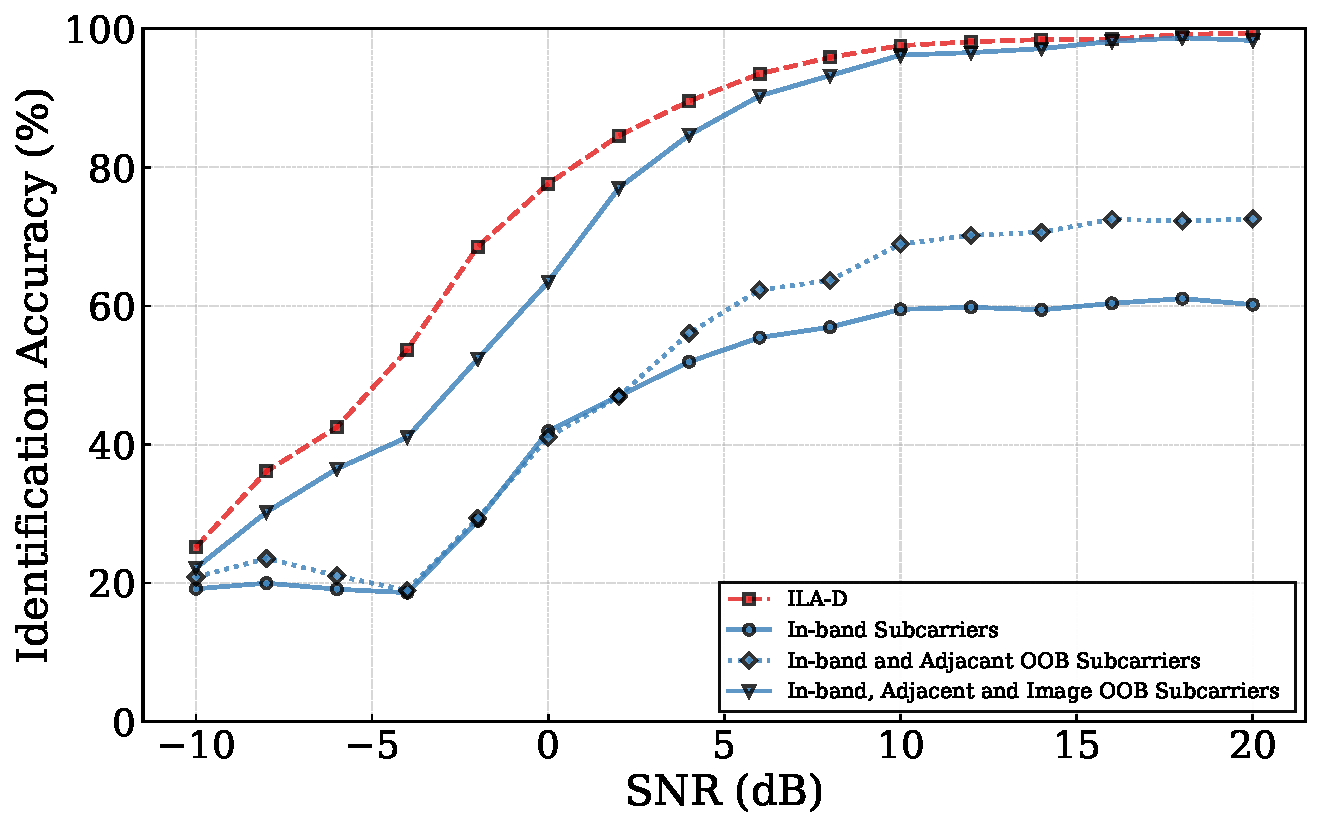
\includegraphics[width=0.8\linewidth]{fig/accuracy_comparison_among_different_input_carriers.pdf}
    \caption{Identification accuracy comparison between ILA-D and region-cropping schemes.}
    \label{fig:partial_subcarrier_accuracy}
\end{figure}


\nc{Experiment and Results, Comparison with Existing Method, Page 11}
{\textit{Comparison with Region-cropping Schemes:}
Region-cropping is a common strategy to reduce input dimensions by retaining selected informative subcarriers.
However, directly selecting subcarriers cannot distinguish physically meaningful interactions from irrelevant interactions among retained subcarriers.
Therefore, we compare ILA-D with three region-cropping baselines, including (i) In-Band subcarriers, (ii) In-Band and adjacent OOB leakage subcarriers, and (iii) In-Band, adjacent OOB, and image OOB leakage subcarriers.
All baselines use the same DDPM framework and experimental settings as ILA-D.

As shown in Fig.~\ref{fig:partial_subcarrier_accuracy}, ILA-D consistently achieves higher identification accuracy under different SNR conditions. Specifically, ILA-D achieves more than 15\% identification accuracy improvement at 0 dB SNR.
The results demonstrate that impairment-guided attention is more effective than directly selecting leakage-related subcarriers because it preserves physically meaningful subcarrier interactions while suppressing irrelevant correlations.}
}



\secc{Comment 5:}{The discussion on why OOB subcarriers improve denoising is not rigorous enough. The current derivation only considers the case of adding a single OOB subcarrier, but the conclusion is then extended to multiple OOB subcarriers without sufficient justification. The paper should provide a more general proof for arbitrary numbers of OOB subcarriers or revise the claim accordingly.}

\secr{Response:}{Thank you for the valuable comment. We agree that the original derivation only considered the case of adding a single OOB subcarrier and did not sufficiently justify the conclusion for multiple OOB observations.
Therefore, we have extended the analysis to an arbitrary number of added OOB subcarriers.

The fundamental reason why adding arbitrary numbers of OOB observations cannot degrade the optimal DDPM denoising performance is that the augmented predictor has a larger hypothesis space. Specifically, the predictor with additional OOB observations can always ignore these added inputs and reproduce any solution achievable by the original in-band predictor. Therefore, the minimum achievable noise prediction loss with additional OOB observations is theoretically no larger than that using only in-band observations.

For an arbitrary integer $M\geq1$, let $\boldsymbol{z}_{t}^{[M]}$ denote $M$ added OOB observations. The augmented input is defined as

\begin{equation}
\boldsymbol{x}_{t}^{[d+M]}
=
[
(\boldsymbol{x}_{t}^{[d]})^{T},
(\boldsymbol{z}_{t}^{[M]})^{T}
]^{T}.
\end{equation}

For any parameter $\theta\in\Theta_d$, there exists an equivalent parameter mapping $I_M(\theta)\in\Theta_{d+M}$ such that

\begin{equation}
\epsilon_{I_M(\theta)}
(\boldsymbol{x}_{t}^{[d+M]},t)
=
\epsilon_{\theta}
(\boldsymbol{x}_{t}^{[d]},t).
\end{equation}

Therefore,

\begin{equation}
\min_{\phi\in\Theta_{d+M}}
\mathcal{L}_{d+M}(\phi)
\leq
\min_{\theta\in\Theta_d}
\mathcal{L}_{d}(\theta).
\end{equation}

Since $M$ is arbitrary, this inequality holds for any number of added OOB observations.

Furthermore, increasing $M$ does not necessarily lead to unlimited performance improvement. The theoretical analysis only guarantees that additional OOB observations cannot increase the minimum achievable loss. In practice, informative OOB observations can provide additional impairment-related information and further improve denoising performance, while redundant observations may lead to diminishing improvement.

The complete proof has been added to the revised manuscript.

\nc{Discussion, OOB-Aided Denoising Advantage Analysis, Page 8}
{
This subsection analyzes why adding physically meaningful OOB leakage subcarriers can improve DDPM-based denoising.
Let $\boldsymbol{x}_{t}^{[d]}\in\mathbb{C}^{d}$ denote the in-band DDPM input.
For an arbitrary integer $M\geq 1$, let $\boldsymbol{z}_{t}^{[M]}\in\mathbb{C}^{M}$ contain $M$ OOB observations.
The augmented input is defined as
\begin{equation}
\boldsymbol{x}_{t}^{[d+M]}
=
\left[
\left(\boldsymbol{x}_{t}^{[d]}\right)^{T},
\left(\boldsymbol{z}_{t}^{[M]}\right)^{T}
\right]^{T}
\in\mathbb{C}^{d+M}.
\tag{45}
\end{equation}

To ensure a fair comparison, both predictors estimate the same $d$ in-band target noise components, denoted by $\boldsymbol{\epsilon}\in\mathbb{C}^{d}$.
Let $\Theta_d$ denote the parameter space of the in-band predictor.
Its DDPM noise-prediction loss is
\begin{equation}
\mathcal{L}_{d}(\theta)
=
\mathbb{E}_{\boldsymbol{x}_0,\boldsymbol{\epsilon},t}
\left[
\left\|
\boldsymbol{\epsilon}
-
\boldsymbol{\epsilon}_{\theta}
\left(\boldsymbol{x}_{t}^{[d]},t\right)
\right\|^{2}
\right],
\qquad
\theta\in\Theta_d.
\tag{46}
\label{eq:main_low_dim_loss}
\end{equation}

Similarly, let $\Theta_{d+M}$ denote the parameter space of the predictor using the augmented input.
Its loss is
\begin{equation}
\mathcal{L}_{d+M}(\phi)
=
\mathbb{E}_{\boldsymbol{x}_0,\boldsymbol{\epsilon},t}
\left[
\left\|
\boldsymbol{\epsilon}
-
\boldsymbol{\epsilon}_{\phi}
\left(\boldsymbol{x}_{t}^{[d+M]},t\right)
\right\|^{2}
\right],
\qquad
\phi\in\Theta_{d+M}.
\tag{47}
\label{eq:main_high_dim_loss}
\end{equation}

The augmented predictor can reproduce any in-band predictor by ignoring all $M$ added OOB observations.
Specifically, for any $\theta\in\Theta_d$, there exists a feasible parameter embedding $\phi=I_M(\theta)\in\Theta_{d+M}$ such that
\begin{equation}
\boldsymbol{\epsilon}_{I_M(\theta)}
\left(\boldsymbol{x}_{t}^{[d+M]},t\right)
=
\boldsymbol{\epsilon}_{\theta}
\left(\boldsymbol{x}_{t}^{[d]},t\right).
\tag{48}
\label{eq:main_parameter_embedding}
\end{equation}
Therefore,
\begin{equation}
\mathcal{L}_{d+M}\left(I_M(\theta)\right)
=
\mathcal{L}_{d}(\theta).
\tag{49}
\label{eq:main_loss_equal_embedding}
\end{equation}

Let $\theta_d^{*}$ be an optimal parameter of the in-band predictor.
Since $I_M(\theta_d^{*})$ is feasible for the augmented predictor, we have
\begin{equation}
\begin{aligned}
\min_{\phi\in\Theta_{d+M}}
\mathcal{L}_{d+M}(\phi)
&\leq
\mathcal{L}_{d+M}\left(I_M(\theta_d^{*})\right) \\
&=
\mathcal{L}_{d}(\theta_d^{*}) \\
&=
\min_{\theta\in\Theta_d}
\mathcal{L}_{d}(\theta).
\end{aligned}
\tag{50}
\label{eq:main_loss_inequality_theta}
\end{equation}

Since $M$ is arbitrary, this inequality holds for any number of added OOB subcarriers.
It shows that adding OOB observations does not increase the minimum achievable noise-prediction loss because the augmented predictor can always ignore uninformative observations.
When the added subcarriers contain impairment leakage correlated with the in-band signal, they provide additional information that may further reduce the noise-prediction loss.
According to the reverse denoising process, more accurate noise prediction can produce a cleaner recovered signal while preserving transmitter-specific impairment features.
Therefore, physically meaningful OOB leakage subcarriers can improve DDPM-based RFF denoising.}
}



\secc{Comment 6:}{Fig. 6 relies mainly on visual inspection to discuss residual noise, proper recovery, and feature drift. The evidence is too qualitative, and the constellation plots alone do not make the claimed differences sufficiently clear.
}

\secr{Response:}{Thank you for this valuable comment. We agree that the original discussion mainly relied on qualitative observation of constellation diagrams and lacked quantitative evaluation.

To provide a more objective analysis, we introduce the peak signal-to-noise ratio (PSNR) as an additional quantitative metric to evaluate the recovered signal quality under different denoising steps.

PSNR measures the reconstruction fidelity between the denoised signal and the clean reference signal:

\begin{equation}
\mathrm{PSNR}
=
10\log_{10}
\left(
\frac{P_{\max}^{2}}
{\mathrm{MSE}}
\right),
\end{equation}

where $P_{\max}$ represents the peak amplitude of the clean reference signal and MSE denotes the mean squared error between the denoised signal and the clean reference signal.

Since the clean reference preserves the transmitter-specific RF impairments used for identification, PSNR reflects both residual noise suppression and distortion introduced by excessive denoising.

Based on PSNR evaluation, the denoising step can be selected quantitatively rather than only through visual inspection. Specifically, PSNR initially increases as denoising removes residual noise. After reaching an appropriate denoising level, excessive denoising may distort subtle transmitter-specific impairment features, resulting in decreased PSNR.

We have revised Fig.~\ref{fig:denoised_performance} by calculating the PSNR value of each constellation subplot and marking the corresponding value directly on each subplot. The updated figure provides both visual and quantitative evidence for the selection of denoising steps.

To clarify it, we have improved the paper as follows.


\setcounter{figure}{5}
\begin{figure}
    \centering
    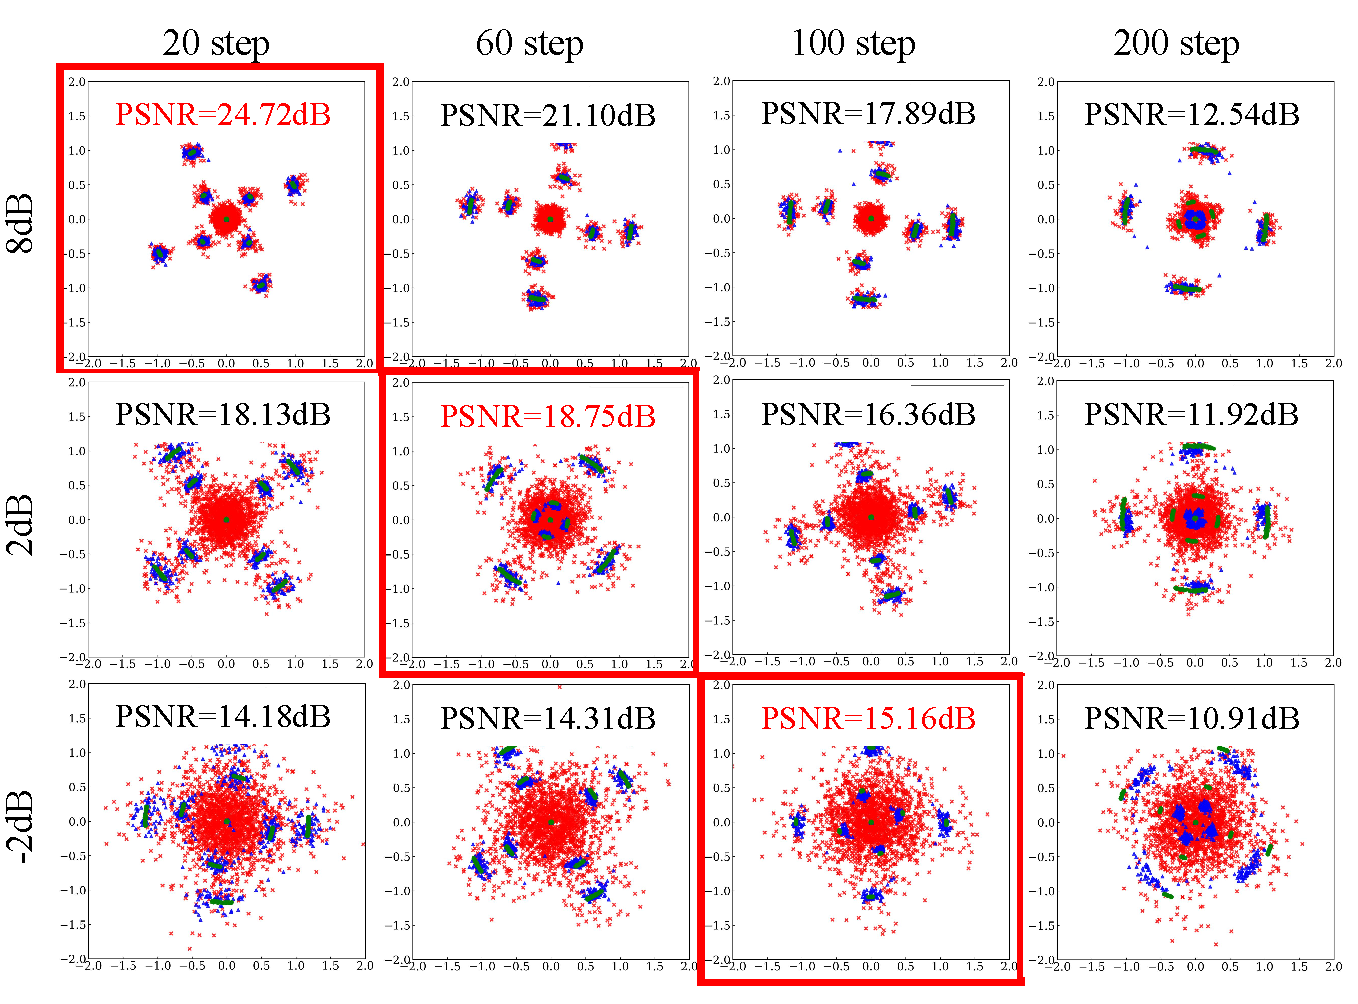
\includegraphics[width=0.8\linewidth]{fig/denoised_performance.pdf}
    \caption{Denoised constellation under different denoising steps.}
    \label{fig:denoised_performance}
\end{figure}

\nc{Experiment and Results, Parameter Sensitivity under Different Settings, Page 9}
{
    The denoising step determines the trade-off between residual noise suppression and the preservation of transmitter-specific RF impairments. To quantitatively evaluate the recovered signal quality, we introduce the peak signal-to-noise ratio (PSNR) as an objective metric. PSNR measures the reconstruction fidelity between the denoised signal and its clean reference, with a higher value indicating better recovery quality. As shown in Fig.~\ref{fig:denoised_performance}, the red, blue, and green points represent the noisy, denoised, and clean samples without noise. Each constellation diagram is annotated with its corresponding PSNR value. PSNR initially increases with the number of denoising steps as the residual noise is gradually removed. However, beyond an appropriate number of steps, excessive denoising may distort subtle RF impairment features, causing the recovered signal to deviate from the clean reference and consequently reducing PSNR.
}
}


\clearpage

%%%%%%%%%%%%%%%%%%%%%%%%%%%%%%%%%%%%%%%%%%%%%%%%%%%%%%%%%%%%%%%%%%%%%%
% response to reviewer 2
%%%%%%%%%%%%%%%%%%%%%%%%%%%%%%%%%%%%%%%%%%%%%%%%%%%%%%%%%%%%%%%%%%%%%%

\begin{center}
\textbf{\Large{IEEE Transactions on Dependable and Secure Computing\\
Manuscript ID: TDSC-2026-05-2030 \\
\vspace{0.3cm} Authors' Response to Reviewer 2}}
\end{center}
	
\secc{Comment 1:}{This manuscript addresses an important problem in low-SNR RF fingerprinting and proposes a physically motivated denoising framework that exploits out-of-band impairment leakage together with diffusion-based noise suppression. The idea of incorporating RF impairment priors into the attention design is interesting, and the experimental results show promising improvements in identification accuracy and computational efficiency. However, the current manuscript still has several limitations that should be addressed.}

\secr{Response:}{Thank you for your insightful review of our paper. We appreciate your recognition of our work. In the following, we provide point-by-point responses and revisions regarding the limitations of this study. 
}

\secc{Comment 2:}{There are some typos and grammar errors should be fixed.\\
(1) $E[\|X\|]^2$ in equition (4) should be presumably be $E[\|X\|^2]$for a power definition.\\
(2) ``Internet of Things (IoTs) networks'' should be ``Internet of Things (IoT) networks''.\\
(3)``such methods require to change existing physical-layer protocols'' should be ``such methods require changes to existing physical-layer protocols''.\\
(4) ``where $\theta$ is learnable parameter'' should be ``where $\theta$ is a learnable parameter''.\\
(5) ``ILA-aided Noise Perdiction Network'' in Fig. 2 should be corrected to ``ILA-aided Noise Prediction Network''.\\
In addition, the font size of several labels is too small, and some workflow details become difficult to read after the figure is scaled to the double-column format.
}

\setcounter{figure}{1}
\begin{figure}[t]
    \centering
    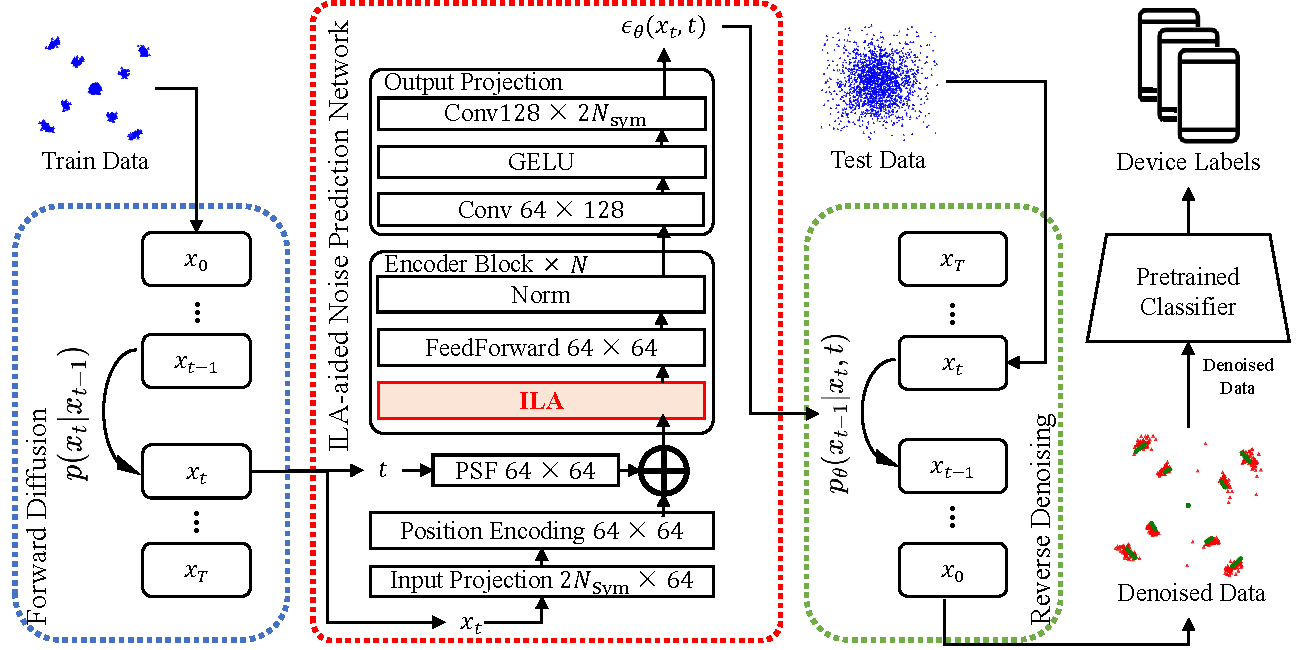
\includegraphics[width=0.9\linewidth]{fig/Overview.pdf}
    \caption{Overview of ILA-D Enhanced RFF Identification.}
    \label{fig:TFP-CDM overview}
\end{figure}

\setcounter{figure}{9}
\begin{figure}[t]
  \centering
  \begin{subfigure}{0.49\textwidth}
    \centering
    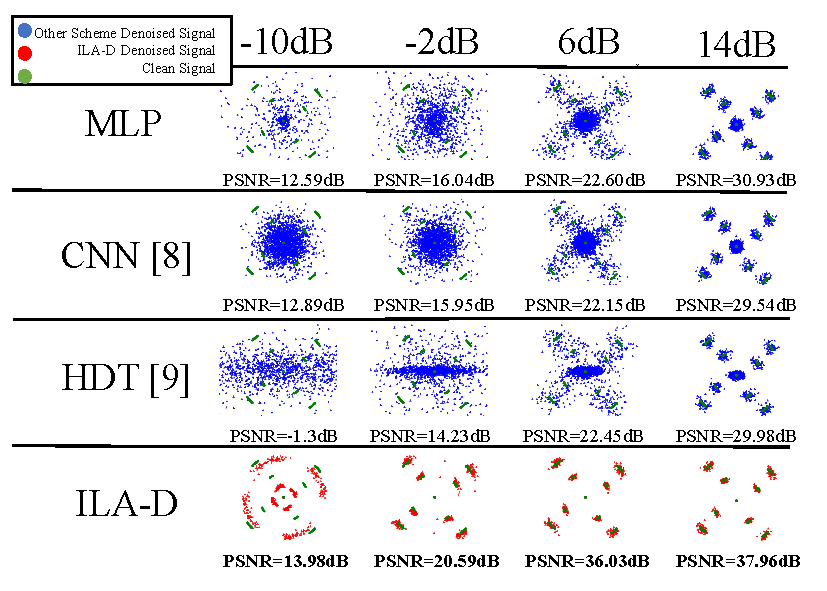
\includegraphics[width=\textwidth]{fig/denoising_constellation_comparison.pdf}
    \caption{}
  \end{subfigure}
  \hfill
  \begin{subfigure}{0.49\textwidth}
    \centering
    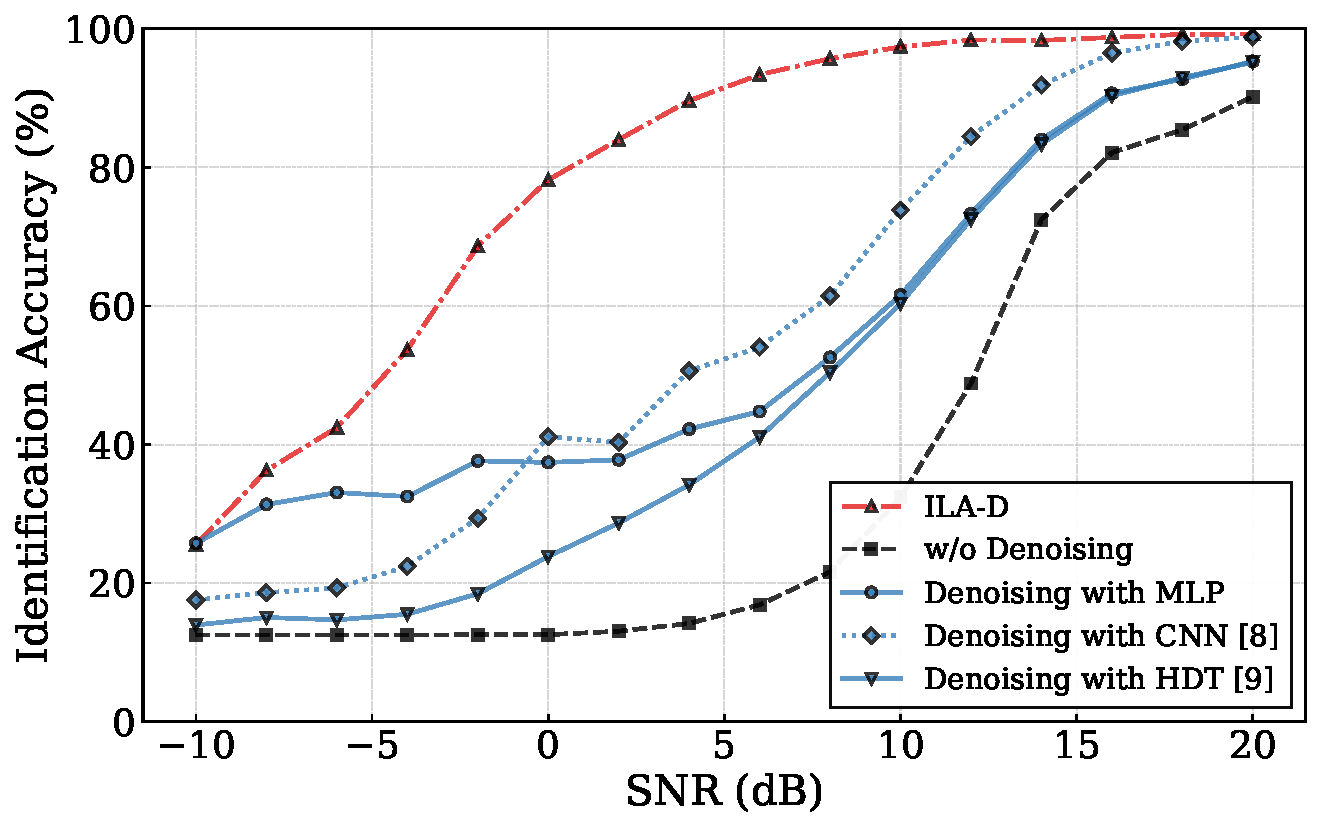
\includegraphics[width=\textwidth]{fig/accuracy_comparison_among_different_denoising_schemes.pdf}
    \caption{}
  \end{subfigure}
  
  \caption{Comparison of different denoising schemes: (a) Denoised constellation (b) Identification accuracy.}
  \label{fig:Comparison of the denoising performance of different schemes: (a) constellation diagrams; (b) confusion matrices.}
\end{figure}


\secr{Response:}{Thank you for your comment. We have revised typos and grammatical errors. We adjusted the font sizes of labels in Fig.~\ref{fig:TFP-CDM overview} and Fig.~\ref{fig:Comparison of the denoising performance of different schemes: (a) constellation diagrams; (b) confusion matrices.}. Furthermore, we converted Fig.~\ref{fig:TFP-CDM overview} to a two-column spanning layout.

To clarify it, we have improved the paper as follows.

\nc{RFF Identification Model and Problem Statement, Page 3}
{Since the considered RF impairments cause only a small change in the total signal power, the in-band SNR $\rho$ is approximated using the ideal signal power:
\begin{equation}
\rho = \frac{P_s}{P_w}
= \frac{\mathbb{E}[\|\boldsymbol{X}\|^2]}
{|\mathcal{K}|\sigma^2},
\label{eq:SNR}
\tag{4}
\end{equation}
where $|\mathcal{K}|$ denotes the number of active subcarriers.
}



\nc{Introduction, Page 1}
{
5G New Radio (NR) supports a wide range of mission-critical communication scenarios, 
such as Internet of Things (IoT) networks~[1], drone communications~[2], and satellite links~[3]. 
}

\nc{Related Work, Noise-robust RFF Identification, Page 2}
{
However, such methods require changes to existing physical-layer protocols, and the additional bandwidth consumption may reduce communication efficiency. 
}


\nc{Overview of Impairment Leakage Attention-based Denoising, Page 4}
{
The training objective minimizes the discrepancy between the true diffusion noise and the predicted noise:
\begin{equation}
\mathcal{L}
=
\mathbb{E}_{\boldsymbol x_0,\boldsymbol \epsilon,t}
\left[
\left\|
\boldsymbol \epsilon-\boldsymbol \epsilon_{\theta}(x_t,t)
\right\|^2
\right],
\tag{15}
\label{eq:diff_loss}
\end{equation}
where $\theta$ is a learnable parameter.
}


\nc{Overview of Impairment Leakage Attention-based Denoising, Page 4}
{As illustrated in Fig.~\ref{fig:TFP-CDM overview}, the ILA-D enhanced RFF identification system consists of four main components: forward diffusion, reverse denoising, an ILA-aided noise prediction network, and a pretrained classifier. 
}



\nc{Experiment and Results, Page 11}
{ 
Fig.~\ref{fig:Comparison of the denoising performance of different schemes: (a) constellation diagrams; (b) confusion matrices.} (a)
compares the denoised constellations. 
To quantitatively compare the denoising performance of different schemes, we use PSNR to evaluate the signals recovered from noisy inputs at different SNR levels. As shown in the figure, ILA-D achieves a higher post-denoising PSNR than the compared baseline methods across all evaluated input SNR conditions. Despite this overall advantage, feature drift may still occur in ILA-D under extremely low-SNR conditions. Severe noise may obscure the original device-specific impairment features, causing the denoising trajectory to shift toward the feature distribution of another device.
}



}



\secc{Comment 3:}{The channel model considered in this paper is mainly limited to an AWGN channel. However, practical RFF deployment is often affected by more complex wireless channel conditions, such as multipath fading. The authors are encouraged to discuss the applicability and robustness of the proposed method under realistic channel environments.}

\secr{Response:}{Thank you for this valuable comment. We agree that multipath fading in practical RFF deployments can alter the amplitude and phase of the received signal and thereby interfere with transmitter-fingerprint extraction. We use an AWGN channel in this paper to isolate channel variation and evaluate the ability of ILA-D to suppress noise while preserving hardware-impairment features at low SNR. For practical 5G NR PUSCH signals, the narrow subcarrier spacing and local frequency correlation of the wireless channel can be exploited to suppress the multipath channel response before applying ILA-D.

Specifically, 5G NR FR1 PUSCH commonly uses a subcarrier spacing of $15$ or $30$ kHz. When adjacent subcarriers lie within the same channel coherence bandwidth, they experience approximately the same channel response:
\begin{equation}
H[k+1]\approx H[k].
\label{eq:adjacent_channel_similarity}
\end{equation}
This observation motivates adjacent-subcarrier differential preprocessing. Taking $Y[k+1]/Y[k]$ approximately cancels the common multiplicative channel response without explicitly estimating $H[k]$. At the same time, transmitter impairments modify the signal components on the two subcarriers differently, so their structured leakage relationships remain in the differential observation.

We consider only adjacent nonzero QPSK subcarriers within the allocated PUSCH region. Specifically, $k\in\{0,\ldots,K-2\}$ and $k,k+1\in\mathcal{K}$, where $K$ is the total number of subcarriers and $\mathcal{K}\subseteq\{0,\ldots,K-1\}$ denotes the set of active subcarriers allocated to the target UE. The corresponding transmitted symbols satisfy $X[k],X[k+1]\in\mathcal{X}_{\mathrm{QPSK}}=\{(\pm1\pm j)/\sqrt{2}\}$. Therefore, $X[k]\neq0$ and $X[k+1]\neq0$. Under these conditions, the ideal differential symbol is defined as
\begin{equation}
D[k]
=
\frac{X[k+1]}{X[k]}
\in
\{1,-1,j,-j\}.
\end{equation}
We next analyze the differential observations for the three impairment-leakage mechanisms used by ILA-D.

First, for IQ-imbalance-induced image leakage, substituting the model in Eq.~(19) of the revised manuscript into a frequency-selective channel gives
\begin{equation}
Y_{\mathrm{img}}^{(c)}[k]
=
H[k]\left(a_cX[k]+b_cX^{*}[m(k)]\right)+N[k],
\end{equation}
where
\begin{equation}
\begin{aligned}
a_c&=\frac{g_ce^{j\varphi_c}+g_c^{-1}e^{-j\varphi_c}}{4},\\
b_c&=\frac{g_ce^{j\varphi_c}-g_c^{-1}e^{-j\varphi_c}}{4},
\end{aligned}
\end{equation}
and $m(k)=(K-k)\bmod K$ denotes the mirrored-subcarrier index. Applying the adjacent-subcarrier ratio yields
\begin{equation}
\begin{aligned}
R_{\mathrm{img}}^{(c)}[k]
&=
\frac{Y_{\mathrm{img}}^{(c)}[k+1]}
{Y_{\mathrm{img}}^{(c)}[k]}\\
&\approx
\frac{a_cX[k+1]+b_cX^{*}[m(k+1)]}
{a_cX[k]+b_cX^{*}[m(k)]}
+\widetilde{N}_{\mathrm{img}}[k].
\end{aligned}
\end{equation}
Letting $\eta_c=b_c/a_c$, and using a first-order approximation when the image component is smaller than the main component, gives
\begin{equation}
R_{\mathrm{img}}^{(c)}[k]
\approx
D[k]
+\eta_c\frac{X^{*}[m(k+1)]-D[k]X^{*}[m(k)]}{X[k]}
+\widetilde{N}_{\mathrm{img}}[k].
\end{equation}
The common channel response is suppressed, whereas the deviation from the ideal QPSK ratio $D[k]$ remains controlled by the device-dependent IQ-imbalance parameter $\eta_c$ and relates the current subcarrier to its mirrored subcarrier. Thus, the long-range mirrored relationship used by image-leakage attention remains in the differential observation.

Second, for DC-offset-induced central leakage, substituting Eq.~(22) of the revised manuscript gives
\begin{equation}
Y_{\mathrm{cen}}^{(c)}[k]
=
H[k]\left(X[k]+\mathrm{DC}_c\delta[k-k_c]\right)+N[k],
\end{equation}
where $k_c=K/2$ is the center subcarrier. The differential observation becomes
\begin{equation}
R_{\mathrm{cen}}^{(c)}[k]
\approx
\frac{X[k+1]+\mathrm{DC}_c\delta[k+1-k_c]}
{X[k]+\mathrm{DC}_c\delta[k-k_c]}
+\widetilde{N}_{\mathrm{cen}}[k].
\end{equation}
For an adjacent pair that does not contain the center subcarrier, the two impulse terms vanish and $R_{\mathrm{cen}}^{(c)}[k]\approx D[k]+\widetilde{N}_{\mathrm{cen}}[k]$. In contrast, for $k=k_c-1$,
\begin{equation}
R_{\mathrm{cen}}^{(c)}[k_c-1]
\approx
D[k_c-1]
+\frac{\mathrm{DC}_c}{X[k_c-1]}
+\widetilde{N}_{\mathrm{cen}}[k_c-1].
\end{equation}
Therefore, DC offset produces a device-dependent deviation localized around the center subcarrier after the common channel response is suppressed. This localized deviation corresponds to the region used by central-leakage attention.

Finally, for CFO-induced adjacent leakage, substituting Eq.~(26) of the revised manuscript gives
\begin{equation}
Y_{\mathrm{adj}}^{(c)}[k]
=
H[k]\left(F_c[0]X[k]+L_c[k]\right)+N[k],
\end{equation}
where
\begin{equation}
L_c[k]
=
\sum_{\substack{r=0\\r\neq k}}^{K-1}
F_c\left[(k-r)\bmod K\right]X[r]
\end{equation}
is the adjacent-leakage component contributed by the other source subcarriers. The adjacent-subcarrier ratio is
\begin{equation}
R_{\mathrm{adj}}^{(c)}[k]
\approx
\frac{F_c[0]X[k+1]+L_c[k+1]}
{F_c[0]X[k]+L_c[k]}
+\widetilde{N}_{\mathrm{adj}}[k].
\end{equation}
The target subcarriers $k$ and $k+1$ contain different combinations of CFO leakage, so $L_c[k]$ and $L_c[k+1]$ are generally different. Their ratio therefore suppresses the approximately common channel response while retaining the local spreading relationship determined by the device-dependent CFO kernel $F_c[\cdot]$. This relationship is the physical structure modeled by adjacent-leakage attention.

In summary, adjacent-subcarrier differential preprocessing exploits the local frequency correlation of the 5G NR channel to suppress the common multipath response. The resulting observations retain the mirrored relationship of image leakage, the center-localized deviation of central leakage, and the local spreading relationship of adjacent leakage. These three relationships are consistent with the physical regions used to construct the ILA masks. The differential resource grid can therefore be further processed by ILA-D for denoising and RFF identification.


\nc{RFF Identification Model and Problem Statement, Page 3}
{Although an AWGN channel is considered in this paper to isolate the effect of noise, ILA-D can also be applied in multipath environments combined with channel-suppression techniques. Owing to the narrow subcarrier spacing of 5G NR and the local frequency correlation of wireless channels, adjacent subcarriers within the coherence bandwidth experience similar channel responses. Existing differential preprocessing methods can therefore suppress the common channel response while retaining transmitter-specific distortions~[26], [27], after which the channel-suppressed signals can be processed by ILA-D.}
}


\secc{Comment 4:}{Fig.~10(a) only provides a qualitative constellation-based comparison of denoising effects, and the authors should add a unified quantitative metric for a more objective evaluation.}

\secr{Response:}{Thank you for the comment. To provide a unified and objective evaluation of the denoising performance, we added the peak signal-to-noise ratio (PSNR) as a quantitative metric. For each denoising method, PSNR is calculated between the recovered complex baseband signal and its corresponding clean reference:
\begin{equation}
\mathrm{PSNR}
=
10\log_{10}
\left(
\frac{P_{\max}^{2}}{\mathrm{MSE}}
\right),
\end{equation}
where $P_{\max}$ is the peak amplitude of the clean reference signal and $\mathrm{MSE}$ is the mean squared error between the recovered and clean signals. A higher PSNR indicates that the recovered signal is closer to the clean reference.

We added the corresponding PSNR results to the constellation comparison in Fig.~\ref{fig:Comparison of the denoising performance of different schemes: (a) constellation diagrams; (b) confusion matrices.}(a). ILA-D achieves a higher post-denoising PSNR than the compared baseline methods across all evaluated input SNR conditions. These quantitative results are consistent with the constellation observations and confirm the denoising advantage of ILA-D.

To clarify it, we have improved the paper as follows.

\nc{Experiment and Results, Comparison with Existing Method, Page 11}
{Fig.~\ref{fig:Comparison of the denoising performance of different schemes: (a) constellation diagrams; (b) confusion matrices.} (a)
compares the denoised constellations. 
To quantitatively compare the denoising performance of different schemes, we use PSNR to evaluate the signals recovered from noisy inputs at different SNR levels. As shown in the figure, ILA-D achieves a higher post-denoising PSNR than the compared baseline methods across all evaluated input SNR conditions. Despite this overall advantage, feature drift may still occur in ILA-D under extremely low-SNR conditions. Severe noise may obscure the original device-specific impairment features, causing the denoising trajectory to shift toward the feature distribution of another device.
}
}
    
\secc{Comment 5:}{The authors should clarify whether the randomly generated impairment parameters in Table I are fixed for each device across training and testing, and whether different random seeds would affect the relative performance ranking of the compared methods.}

\secr{Response:}{Thank you for this valuable comment. The impairment parameters of each simulated device are randomly sampled once from the ranges in Table~I and remain fixed for that device across both training and testing.

To evaluate the influence of random seeds, we generated 32 simulated devices with different impairment parameters and divided them into four device groups. Independent experiments were conducted on each group using the same compared denoising schemes, and Fig.~\ref{fig:Comparison of the denoising performance of different schemes: (a) constellation diagrams; (b) confusion matrices.} reports the average results across the four groups. ILA-D consistently achieves higher identification accuracy across the evaluated SNR range, indicating that the relative performance advantage remains stable under different random seeds and device impairment realizations.
To clarify it, we have improved the paper as follows.

\nc{Experiment and Results, Experimental Setup, Page 9}
{Based on this impairment model, 8 devices with distinct impairment parameters are randomly generated. For each device, these impairment parameters are sampled once from the ranges in Tab.~I and remain fixed across both training and testing.}

\nc{Experiment and Results, Comparison with Existing Method, Page 11}
{As shown in Fig.~\ref{fig:Comparison of the denoising performance of different schemes: (a) constellation diagrams; (b) confusion matrices.} (b), ILA-D consistently outperforms the CNN and HDT schemes. To reduce the experimental uncertainty associated with a single group of simulated devices, we independently generate four device groups, repeat the evaluation for each group, and report the mean identification accuracy across all groups. ILA-D achieves an identification accuracy gain of more than $37.06\%$ at 0 dB. It also maintains a clear advantage over MLP when $\mathrm{SNR}>-8$ dB, while their performance becomes comparable under more severe noise conditions. This advantage comes from the ability of ILA-D to explicitly model both local and long-range dependencies between in-band subcarriers and their leakage positions. MLP mixes the input features through fully connected layers and therefore needs to learn these structured frequency-domain relationships implicitly.
}
}
   

\secc{Comment 6:}{The paper reports throughput and memory reduction, but the authors should specify batch size, precision type, GPU memory setting, and whether timing includes only the denoising network or the whole pipeline.
}

\secr{Response:}{Thank you for this valuable comment. We have clarified the experimental settings and measurement scope for the reported throughput and GPU memory cost.

All efficiency experiments were conducted on an NVIDIA Tesla V100 PCIe GPU using the default PyTorch floating-point precision, i.e., FP32. For the throughput evaluation, the batch size was set to 64, and each sample contained 10 OFDM symbols and 180 subcarriers. The timing includes only the complete reverse denoising process, including all denoising steps and the corresponding noise-prediction network executions. 

The throughput in the figure is measured in batches per second and calculated as $\mathcal{T}_{\mathrm{batch}}=N_{\mathrm{batch}}/T_{\mathrm{den}}$, where $N_{\mathrm{batch}}$ is the number of processed batches and $T_{\mathrm{den}}$ is the total reverse-denoising time. We evaluate throughput at different SNR levels because lower-SNR signals require more reverse-denoising steps, resulting in lower throughput.

The reported GPU memory cost is the peak memory usage during model training. It includes the denoising model, loaded training data, forward diffusion, and the intermediate tensors and other memory allocations generated during training. We evaluate the effects of both batch size and input subcarrier length. For the batch-size evaluation, each sample contained 10 OFDM symbols and 180 subcarriers, while the number of slots processed simultaneously was varied. For the subcarrier-length evaluation, the batch size was fixed at 64, and each sample contained 10 OFDM symbols, while the number of input subcarriers was varied. These experiments evaluate the memory cost with respect to the number of concurrently processed slots and the input subcarrier length, respectively.

To clarify it, we have improved the paper as follows.

\nc{Experiment and Results, Efficiency Comparison, Page 12}
{
All efficiency experiments are conducted on an NVIDIA Tesla V100 PCIe GPU using FP32 precision.

\textit{Denoising Throughput}: Fig.~12 compares the denoising throughput of different schemes. 
Each batch contains 64 slots, with each slot consisting of 10 OFDM symbols and 180 subcarriers. 
The timing covers only the reverse denoising process, and the throughput is calculated as $\mathcal{T}_{\mathrm{batch}}=N_{\mathrm{batch}}/T_{\mathrm{den}}$ batches per second.

Throughput increases with SNR because higher-SNR signals require fewer denoising iterations. 
ILA-D achieves about $4.26\times$ the throughput of global attention. 
It also retains about $0.79\times$ the throughput of the baselines with smaller attention regions while providing better identification accuracy, showing a favorable efficiency--accuracy trade-off.

Fig.~12 marks the batch-rate requirements converted from the maximum slot rates for 15 kHz and 30 kHz FR1 SCS according to 3GPP TS 38.211 Release 19. 
ILA-D satisfies these requirements when $\mathrm{SNR}\geq -4$ dB.

\textit{Denoising Memory Cost}: The reported memory cost is the peak GPU memory usage during training, including the model, input data, forward diffusion, and other training-related allocations.

Fig.~13 evaluates the effect of the number of concurrently processed slots, where each slot contains 10 OFDM symbols and 180 subcarriers. 
Memory consumption increases with the number of slots because more samples are processed in parallel. 
Compared with global attention, ILA-D reduces memory consumption by about $80.35\%$, allowing more slots to be processed under the same hardware constraint.

Fig.~14 evaluates the effect of the input subcarrier length with a fixed batch size of 64. 
Memory consumption increases with the number of input subcarriers.
Compared with global attention, ILA-D reduces memory consumption by about $83.67\%$. 
It also maintains a memory cost close to the region cropping baselines while achieving better identification accuracy, showing a favorable performance--memory trade-off.
}
}

\clearpage

%%%%%%%%%%%%%%%%%%%%%%%%%%%%%%%%%%%%%%%%%%%%%%%%%%%%%%%%%%%%%%%%%%%%%%
% response to reviewer 3
%%%%%%%%%%%%%%%%%%%%%%%%%%%%%%%%%%%%%%%%%%%%%%%%%%%%%%%%%%%%%%%%%%%%%%

\begin{center}
\textbf{\Large{IEEE Transactions on Dependable and Secure Computing\\
Manuscript ID: TDSC-2026-05-2030 \\
\vspace{0.3cm} Authors' Response to Reviewer 3}}
\end{center}

\secc{Comment 1:}{In the Introduction, when the concept of estimating on Out Of Band subcarriers, could you please clarify what is meant by out of band? Does it mean sensing data in carriers that are still usable within a 5G framework but not used at that particular moment by the device? Or is there a broader spectral mask around the standard set of carriers to observe all the time, and if so how broad is that mask?
}

\secr{Response:}{Thank you for this valuable comment. In this paper, OOB refers to the inactive PRBs outside the PUSCH allocation of the target UE but still within the resource grid. These PRBs carry no intended data from the UE but may contain RF-impairment leakage. No additional spectral mask outside the configured NR carrier is required. 

To clarify it, we have improved the paper as follows.

\nc{Introduction, footnote, Page 1}
{In this paper, OOB refers to inactive subcarriers outside the PUSCH PRBs allocated to the target UE but within the NR resource grid.}
}

\secc{Comment 2:}{It is mentioned that the paper expands a contribution from ICC, but would it be possible for completeness to provide a public reference, even a simple Arxiv paper of that past contribution?
}

\secr{Response:}{Thank you for this helpful suggestion. We have added a public reference to our previous ICC contribution in the revised manuscript.

To clarify it, we have improved the paper as follows.

\nc{Introduction, Page 2}
{This paper extends our ICC workshop version~[10]. 
We additionally take efficiency under consideration, 
ensuring high throughput and low memory consumption
while preserving transmitter-specific impairment features during denoising.
}
}

\secc{Comment 3:}{Notation: below equation 2 the quantity $F_{i,j}$ is mentioned in the text but does not appear in the equations? Then in the definition of the SNR, should the power be of $X$ or of $\tilde X$ accounting for the impairments? Also, still in (4) what is the absolute value of $K$ at the denominator?}

\secr{Response:}{Thank you for pointing out these notation issues. We have revised the manuscript to clarify three points: (i) the relationship between $F_{i,j}$ and $\boldsymbol{F}_c$, (ii) the use of the ideal signal power in the SNR definition, and (iii) the meaning of $|\mathcal{K}|$ in the noise-power term.

First, $F_{i,j}$ is the $(i,j)$-th element of the impairment matrix:
\begin{equation}
\boldsymbol{F}_c
=
[F_{i,j}]_{i,j=0}^{K-1}
\in
\mathbb{C}^{K\times K}.
\end{equation}

Second, we use $\mathbb{E}[\|\boldsymbol{X}\|^2]$ as the signal power in the SNR definition. At a high level, Eq.~(4) defines the nominal SNR used to control the AWGN level during dataset generation, rather than an online SNR estimate obtained from the received waveform. The normalized ideal waveform provides the same reference power for all devices. In contrast, using $\mathbb{E}[\|\tilde{\boldsymbol{X}}\|^2]$ would make the nominal SNR depend on the device-specific impairment parameters, thereby coupling the controlled noise level with the RF fingerprint strength.

Moreover, the considered RF impairments cause only a limited change in the average power of the active subcarriers. We verify this by comparing the ideal power with the power after RF impairment but before AWGN. For device $c$, the latter is calculated as
\begin{equation}
P_{\tilde{X},c}
=
\frac{1}{N_{\mathrm{sym}}|\mathcal K|}
\sum_{n=1}^{N_{\mathrm{sym}}}
\sum_{k\in\mathcal K}
\left|\tilde X_c[k,n]\right|^2,
\end{equation}
whereas the normalized QPSK waveform satisfies
\begin{equation}
P_X
=
\frac{1}{N_{\mathrm{sym}}|\mathcal K|}
\sum_{n=1}^{N_{\mathrm{sym}}}
\sum_{k\in\mathcal K}
|X[k,n]|^2
=1.
\end{equation}
Using $N_{\mathrm{sym}}=2000$ OFDM symbols for each of the eight simulated devices, the average difference is calculated in the power domain as
\begin{equation}
\Delta_{\mathrm{avg}}
=
10\log_{10}
\left(
\frac{
\frac{1}{8}\sum_{c=1}^{8}P_{\tilde{X},c}
}{P_X}
\right)
=1.09~\mathrm{dB}.
\end{equation}
This result confirms that the ideal and impairment-affected active-subcarrier powers remain close under the considered settings. Therefore, using the ideal waveform provides a consistent SNR reference across devices without materially changing the evaluated noise condition.

The relationship between the ideal and impaired signal powers is further derived below from the IQ imbalance, DC offset, and CFO models.

For IQ imbalance, the impaired frequency-domain signal is
\begin{equation}
\begin{aligned}
X_{BB}^{rv}[k]
&=
\frac{g e^{j\varphi}+g^{-1}e^{-j\varphi}}{4}X_{BB}[k]
\\
&\quad+
\frac{g e^{j\varphi}-g^{-1}e^{-j\varphi}}{4}
X_{BB}^*[m(k)],
\end{aligned}
\end{equation}
where $m(k)=(K-k)\bmod K$ is the mirrored-subcarrier index. After compensating for the common receiver gain, this expression can be written as
\begin{equation}
X_{\mathrm{IQ}}[k]
=
aX[k]+bX^*[m(k)],
\end{equation}
where
\begin{equation}
a=\frac{g e^{j\varphi}+g^{-1}e^{-j\varphi}}{2},
\qquad
b=\frac{g e^{j\varphi}-g^{-1}e^{-j\varphi}}{2}.
\end{equation}
Its expected power is
\begin{equation}
\begin{aligned}
\mathbb{E}[|X_{\mathrm{IQ}}[k]|^2]
={}&
|a|^2\mathbb{E}[|X[k]|^2]
+
|b|^2\mathbb{E}[|X[m(k)]|^2]
\\
&+
2\operatorname{Re}
\left\{
ab^*\mathbb{E}[X[k]X[m(k)]]
\right\}.
\end{aligned}
\end{equation}
The QPSK symbols transmitted on different active subcarriers are independently generated and have zero mean. Therefore, for $k\neq m(k)$,
\begin{equation}
\mathbb{E}[X[k]X[m(k)]]
=
\mathbb{E}[X[k]]
\mathbb{E}[X[m(k)]]
=
0.
\end{equation}
When $k=m(k)$, uniformly distributed QPSK symbols satisfy $\mathbb{E}[X^2[k]]=0$. Thus, the expected cross term is zero. Since the mirrored-subcarrier mapping is a permutation, summing over all subcarriers gives
\begin{equation}
\begin{aligned}
\mathbb{E}\!\left[\|\boldsymbol{X}_{\mathrm{IQ}}\|^2\right]
&=
\left(|a|^2+|b|^2\right)
\mathbb{E}\!\left[\|\boldsymbol{X}\|^2\right]
\\
&=
\frac{g^2+g^{-2}}{2}
\mathbb{E}\!\left[\|\boldsymbol{X}\|^2\right]
\\
&\approx
\mathbb{E}\!\left[\|\boldsymbol{X}\|^2\right],
\end{aligned}
\end{equation}
where the approximation holds after common-gain compensation and for a small residual amplitude imbalance. The phase imbalance does not change the total expected power.

For DC offset, the impaired signal is
\begin{equation}
\widetilde{X}_{BB}[k]
=
X_{BB}[k]
+
DC\delta[k-k_c].
\end{equation}
Since the QPSK symbols are zero-mean, the expected cross term between the signal and the DC component is zero. Therefore,
\begin{equation}
\mathbb{E}\!\left[\|\boldsymbol{X}_{\mathrm{DC}}\|^2\right]
=
\mathbb{E}\!\left[\|\boldsymbol{X}\|^2\right]
+
|DC|^2
\approx
\mathbb{E}\!\left[\|\boldsymbol{X}\|^2\right],
\end{equation}
where $|DC|^2\leq 0.005$ under our impairment setting.

For CFO, the impaired time-domain signal is
\begin{equation}
x_{BB}^{rv}[n]
=
\frac{1}{2}x_{BB}[n]e^{j2\pi\Delta f nT_s}.
\end{equation}
The factor $1/2$ is included in the common receiver gain compensation. Since $|e^{j2\pi\Delta f nT_s}|=1$, CFO preserves the time-domain signal power. Parseval's theorem then gives
\begin{equation}
\mathbb{E}\!\left[\|\boldsymbol{X}_{\mathrm{CFO}}\|^2\right]
=
\mathbb{E}\!\left[\|\boldsymbol{X}\|^2\right].
\end{equation}

Consequently, under the considered impairment settings,
\begin{equation}
\mathbb{E}\!\left[\|\widetilde{\boldsymbol{X}}\|^2\right]
\approx
\mathbb{E}\!\left[\|\boldsymbol{X}\|^2\right].
\end{equation}
We therefore use the ideal signal power to provide a consistent SNR definition across devices.

Third, we have also clarified that $|\mathcal{K}|$ denotes the number of active subcarriers. Therefore, $|\mathcal{K}|\sigma^2$ represents the total noise power over the active subcarriers.

To clarify it, we have improved the paper as follows.

\nc{RFF Identification Model and Problem Statement, Page 3}
{In practical transmitters, unavoidable hardware impairments, e.g., CFO, IQ imbalance, and DC offset, introduce transmitter-specific distortions to the transmitted signal.
For UE $c \in \mathcal{C}$, the impaired equivalent baseband signal is modeled as:
\begin{equation}
\tilde{\boldsymbol{X}} = \boldsymbol{F}_c \boldsymbol{X}
\tag{2}
\end{equation}
where $\boldsymbol{F}_c = [F_{i,j}]_{i,j=0}^{K-1} \in \mathbb{C}^{K \times K}$ is the transmitter-specific impairment matrix, and $F_{i,j}$ represents the complex gain from the $j$-th ideal subcarrier to the $i$-th impaired subcarrier.
}
\nc{RFF Identification Model and Problem Statement, Page 3}
{
Since the considered RF impairments cause only a small change in the total signal power, the in-band SNR $\rho$ is approximated using the ideal signal power:
\begin{equation}
\rho = \frac{P_s}{P_w}
= \frac{\mathbb{E}[\|\boldsymbol{X}\|^2]}
{|\mathcal{K}|\sigma^2},
\tag{4}
\label{eq:SNR 2}
\end{equation}
where $|\mathcal{K}|$ denotes the number of active subcarriers.}
}


\secc{Comment 4:}{Figure 2 is way too small, please expand it, perhaps to a single column format. The same holds for other figures, e.g. figure 3, 6, 10a
}

\secr{Response:}{Thank you for this helpful comment. We have enlarged Fig.~2, Fig.~3, Fig.~6, and Fig.~10 (a) to improve their readability. In particular, Fig.~2 has been changed to a double-column format.

To clarify it, we have improved the paper as follows.

\setcounter{figure}{1}
\begin{figure}
    \centering
    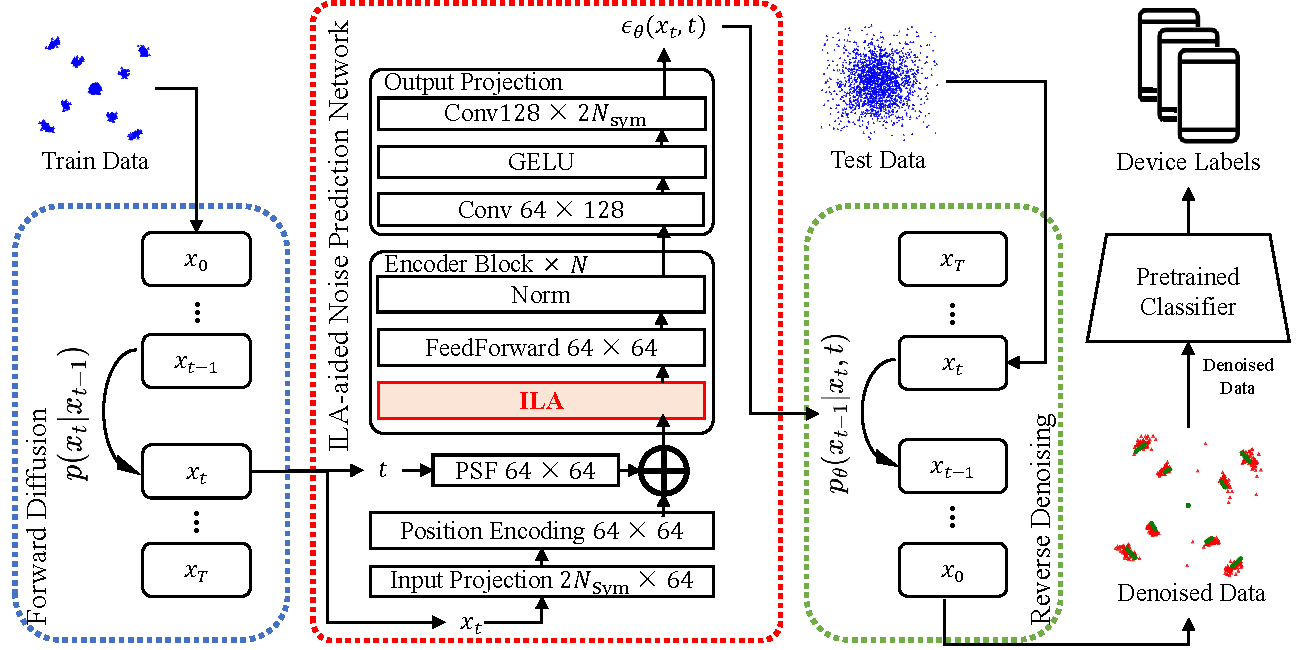
\includegraphics[width=0.8\linewidth]{fig/Overview.pdf}
    \caption{Overview of ILA-D Enhanced RFF Identification.}
    \label{fig:TFP-CDM overview 2}
\end{figure}



\nc{Overview of Impairment Leakage Attention-based Denoising, Fig.~\ref{fig:TFP-CDM overview 2}, Page 5}
{
As illustrated in Fig.~\ref{fig:TFP-CDM overview 2}, the ILA-D enhanced RFF identification system consists of four main components: forward diffusion, reverse denoising, an ILA-aided noise prediction network, and a pretrained classifier. 
}

\setcounter{figure}{2}
\begin{figure}
    \centering
    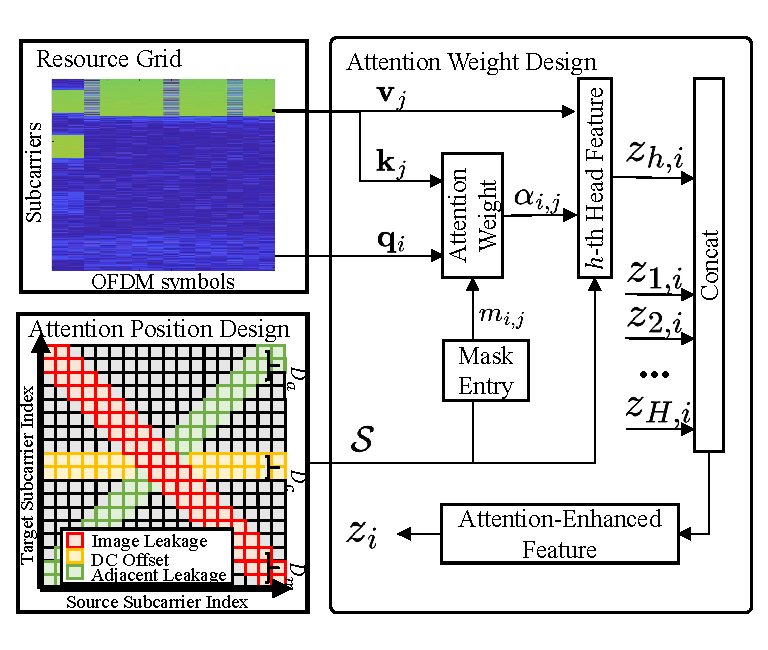
\includegraphics[width=0.6\linewidth]{fig/The structure of impairment-driven fusion attention and its location in Noise Prediction Network.pdf}
    \caption{The structure of Impairment Leakage Attention.}
    \label{fig:The structure of Noise Predictor Network}
\end{figure}


\nc{Design of Impairment Leakage Attention, Fig.~\ref{fig:The structure of Noise Predictor Network}, Page 6}
{
This section introduces Impairment Leakage Attention (ILA). 
ILA retains the standard query-key-value attention and learnable attention weights. It introduces RF impairment priors into attention-position selection. As shown in Fig.~\ref{fig:The structure of Noise Predictor Network}, 
ILA performs leakage-aware attention-position selection and attention-weight assignment to extract attention-enhanced features from a resource-grid-like input.
}

\setcounter{figure}{5}
\begin{figure}
    \centering
    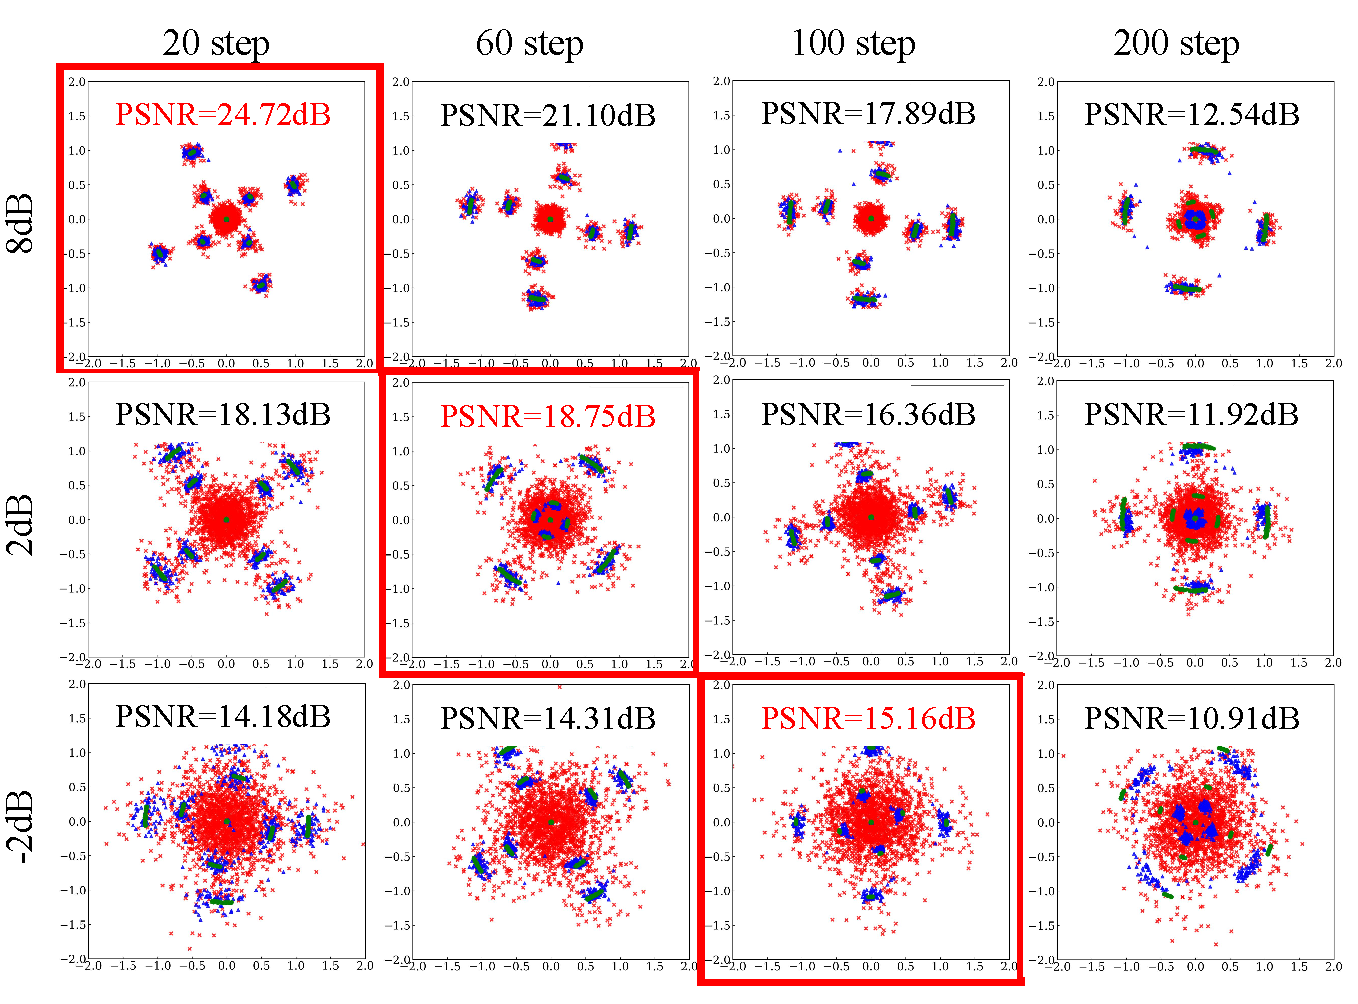
\includegraphics[width=0.75\linewidth]{fig/denoised_performance.pdf}
    \caption{Denoised constellation under different denoising steps.}
    \label{fig:denoised_performance 2}
\end{figure}

\nc{Experiment and Results, Fig.~\ref{fig:denoised_performance 2}, Page 10}
{
As shown in Fig.~\ref{fig:denoised_performance 2}, the red, blue, and green points represent the noisy, denoised, and clean samples without noise. Each constellation diagram is annotated with its corresponding PSNR value. PSNR initially increases with the number of denoising steps as the residual noise is gradually removed. However, beyond an appropriate number of steps, excessive denoising may distort subtle RF impairment features, causing the recovered signal to deviate from the clean reference and consequently reducing PSNR.
}

\setcounter{figure}{9}
\begin{figure*}
  \centering
  \begin{subfigure}{0.49\textwidth}
    \centering
    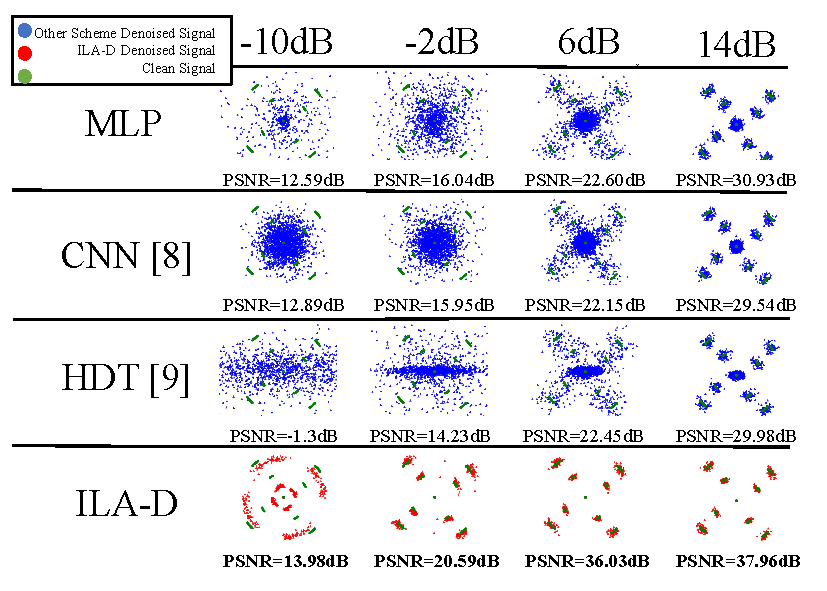
\includegraphics[width=\textwidth]{fig/denoising_constellation_comparison.pdf}
    \caption{}
  \end{subfigure}
  \begin{subfigure}{0.49\textwidth}
    \centering
    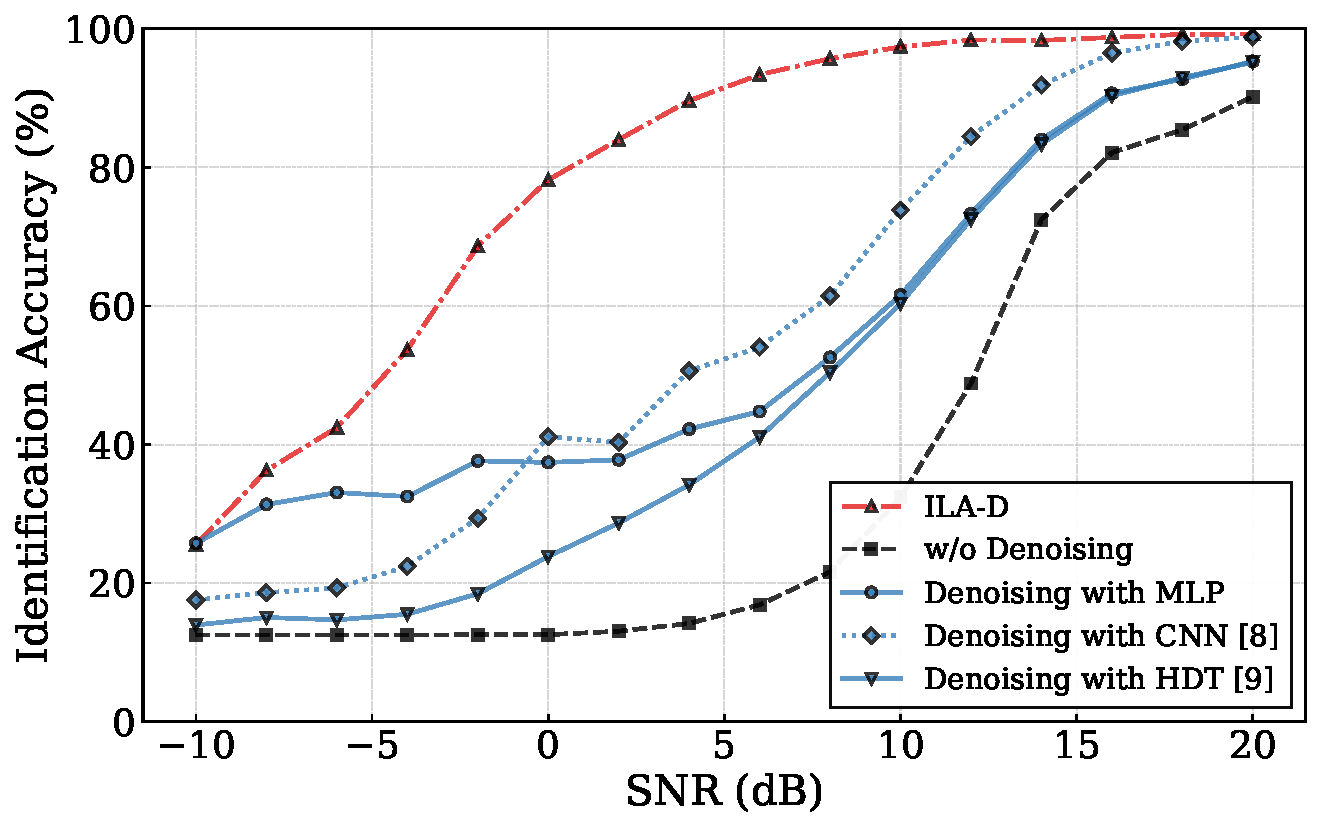
\includegraphics[width=0.95\textwidth]{fig/accuracy_comparison_among_different_denoising_schemes.pdf}
    \caption{}
  \end{subfigure}
  
  \caption{Comparison of different denoising schemes: (a) Denoised constellation (b) Identification accuracy.}
  \label{fig:Comparison of the denoising performance of different schemes 2: (a) constellation diagrams; (b) confusion matrices.}
\end{figure*}

\nc{Experiment and Results, Fig.~\ref{fig:Comparison of the denoising performance of different schemes 2: (a) constellation diagrams; (b) confusion matrices.}, Page 12}
{
Fig.~\ref{fig:Comparison of the denoising performance of different schemes 2: (a) constellation diagrams; (b) confusion matrices.} (a)
compares the denoised constellations. 
To quantitatively compare the denoising performance of different schemes, we use PSNR to evaluate the signals recovered from noisy inputs at different SNR levels. As shown in the figure, ILA-D achieves a higher post-denoising PSNR than the compared baseline methods across all evaluated input SNR conditions. Despite this overall advantage, feature drift may still occur in ILA-D under extremely low-SNR conditions. Severe noise may obscure the original device-specific impairment features, causing the denoising trajectory to shift toward the feature distribution of another device.

As shown in Fig.~\ref{fig:Comparison of the denoising performance of different schemes 2: (a) constellation diagrams; (b) confusion matrices.} (b), ILA-D consistently outperforms the CNN and HDT schemes. To reduce the experimental uncertainty associated with a single group of simulated devices, we independently generate four device groups, repeat the evaluation for each group, and report the mean identification accuracy across all groups. ILA-D achieves an identification accuracy gain of more than $37.06\%$ at 0 dB. It also maintains a clear advantage over MLP when $\mathrm{SNR}>-8$ dB, while their performance becomes comparable under more severe noise conditions. This advantage comes from the ability of ILA-D to explicitly model both local and long-range dependencies between in-band subcarriers and their leakage positions. MLP mixes the input features through fully connected layers and therefore needs to learn these structured frequency-domain relationships implicitly.
}


}

\secc{Comment 5:}{When describing the proposed architecture and signal models for the denoising (forward/reverse) processing and for the ILA module, it would be nice to add a sharper description of what is novel in these and what is instead reused, or readapted from the literature, and in what sense these have been customized to the problem/signals at hand.
}

\secr{Response:}{Thank you for this valuable comment. The main novelty of ILA-D lies in introducing RF impairment leakage priors into diffusion-based RFF denoising. Based on the image, central, and adjacent leakage caused by IQ imbalance, DC offset, and CFO, ILA focuses feature extraction on fingerprint-related subcarrier interactions while avoiding unnecessary computation.

The forward and reverse diffusion processes follow the standard DDPM framework, and the noise-prediction network uses a Transformer encoder backbone. The problem-specific customization lies in the impairment-leakage mask. This mask determines the valid attention positions according to the derived leakage regions, while the attention weights within these regions are learned from data. We have clarified this distinction in the revised manuscript.

To clarify it, we have improved the paper as follows.

\nc{Overview of Impairment Leakage Attention-based Denoising, Page 4}
{The forward diffusion, reverse denoising, and noise-prediction objective follow the standard DDPM framework~[27]. To adapt DDPM to 5G RFF denoising, the clean sample $\boldsymbol{x}_0=\widetilde{\boldsymbol{X}}$ is represented as a complex PUSCH resource grid containing transmitter-specific impairments. The number of reverse denoising steps is further selected according to the estimated SNR of the received signal.}

\nc{Overview of Impairment Leakage Attention-based Denoising, Page 5}
{
The ILA-aided noise prediction network is built on a standard Transformer encoder-only framework~[28], including input projection, positional encoding, timestep conditioning, encoder blocks, and output projection. 
The structure of the ILA-aided noise prediction network is illustrated in Fig.~\ref{fig:TFP-CDM overview 2}.
}

\nc{Design of Impairment Leakage Attention, Page 5}
{
This section introduces Impairment Leakage Attention (ILA). 
ILA retains the standard query-key-value attention and learnable attention weights. It introduces RF impairment priors into attention-position selection. As shown in Fig.~\ref{fig:The structure of Noise Predictor Network}, 
ILA performs leakage-aware attention-position selection and attention-weight assignment to extract attention-enhanced features from a resource-grid-like input.
}

}


\secc{Comment 6:}{I like your analysis that links the leakages with their hardware cause in section V, but if one can construct a deterministic model of what sub-carriers to consider, what is the need of a data driven approach? I understand it is needed to compute weights for each selected subcarrier, but why a transformer/attention like architecture? Could a simpler architecture (MLP?) do the job, with fewer parameters and making it easier to train?
}

\secr{Response:}{Thank you for this insightful comment. We agree that the OOB leakage locations derived from hardware impairment mechanisms provide deterministic physical priors. However, these priors only identify the frequency regions that may contain device-specific information. They cannot determine the actual contribution of each subcarrier under different devices and noise conditions. We therefore use a data-driven attention mechanism to learn the correlations and adaptive weights among the selected subcarriers.

Modeling subcarrier dependencies is important because impairment leakage has a structured relationship with the in-band signal. Adjacent leakage is related to neighboring subcarriers, image leakage is related to mirrored subcarriers, and central leakage is concentrated around the center subcarrier. An MLP can serve as a low-complexity noise predictor, but it does not explicitly model these pairwise frequency-domain relationships. Attention directly assigns input-dependent weights to the associated in-band and leakage subcarriers. To control its computational and memory costs, ILA restricts attention to the leakage regions identified by the physical priors.

We compare ILA-D with an MLP-based noise predictor in Fig.~10 under the same DDPM framework and experimental settings. ILA-D achieves higher identification accuracy across most evaluated SNR conditions, while MLP obtains comparable performance only under extremely low-SNR conditions. These results indicate that an MLP can perform basic denoising, but explicitly modeling structured subcarrier dependencies better preserves device-specific leakage features.

To clarify it, we have improved the paper as follows.

\nc{Design of Impairment Leakage Attention, Attention Weight Assignment, Page 7}
{In Sec.~V-A we have discussed where RF impairment leakage may occur. But it is still needed to quantify the actual contribution of each subcarrier. Therefore, we use data-driven attention to learn the correlations and adaptive weights among the selected subcarriers.}

\nc{Experiment and Results, Comparison with Existing Method, Page 11}
{
As shown in Fig.~\ref{fig:Comparison of the denoising performance of different schemes 2: (a) constellation diagrams; (b) confusion matrices.} (b), ILA-D consistently outperforms the CNN and HDT schemes. To reduce the experimental uncertainty associated with a single group of simulated devices, we independently generate four device groups, repeat the evaluation for each group, and report the mean identification accuracy across all groups. ILA-D achieves an identification accuracy gain of more than $37.06\%$ at 0 dB. It also maintains a clear advantage over MLP when $\mathrm{SNR}>-8$ dB, while their performance becomes comparable under more severe noise conditions. This advantage comes from the ability of ILA-D to explicitly model both local and long-range dependencies between in-band subcarriers and their leakage positions. MLP mixes the input features through fully connected layers and therefore needs to learn these structured frequency-domain relationships implicitly.}
}

\secc{Comment 7:}{In section VI.A, what is the parameters $D_a$ set to 1 and what is its relation to equation 44? Maybe I missed it but $D_a$ does not appear in the relevant equations? And what does it mean that $D_a$ is equal to 1 in terms of adjacent sub-carriers, only 1?
}

\secr{Response:}{Thank you for this comment. $D_a$ controls the radius of the adjacent-leakage attention region. According to Eq.~(44), CFO-induced leakage decreases as the relative subcarrier distance increases. We therefore set $D_a=1$ to retain the strongest adjacent leakage. Specifically, the region contains the source subcarrier and its nearest neighbor on each side, i.e., $\{i-1,i,i+1\}$, with a total width of $2D_a+1=3$. We have clarified this definition and its relation to Eq.~(44) in the revised manuscript.

To clarify it, we have improved the paper as follows.

\setcounter{figure}{4}
\begin{figure}[t]
    \centering
    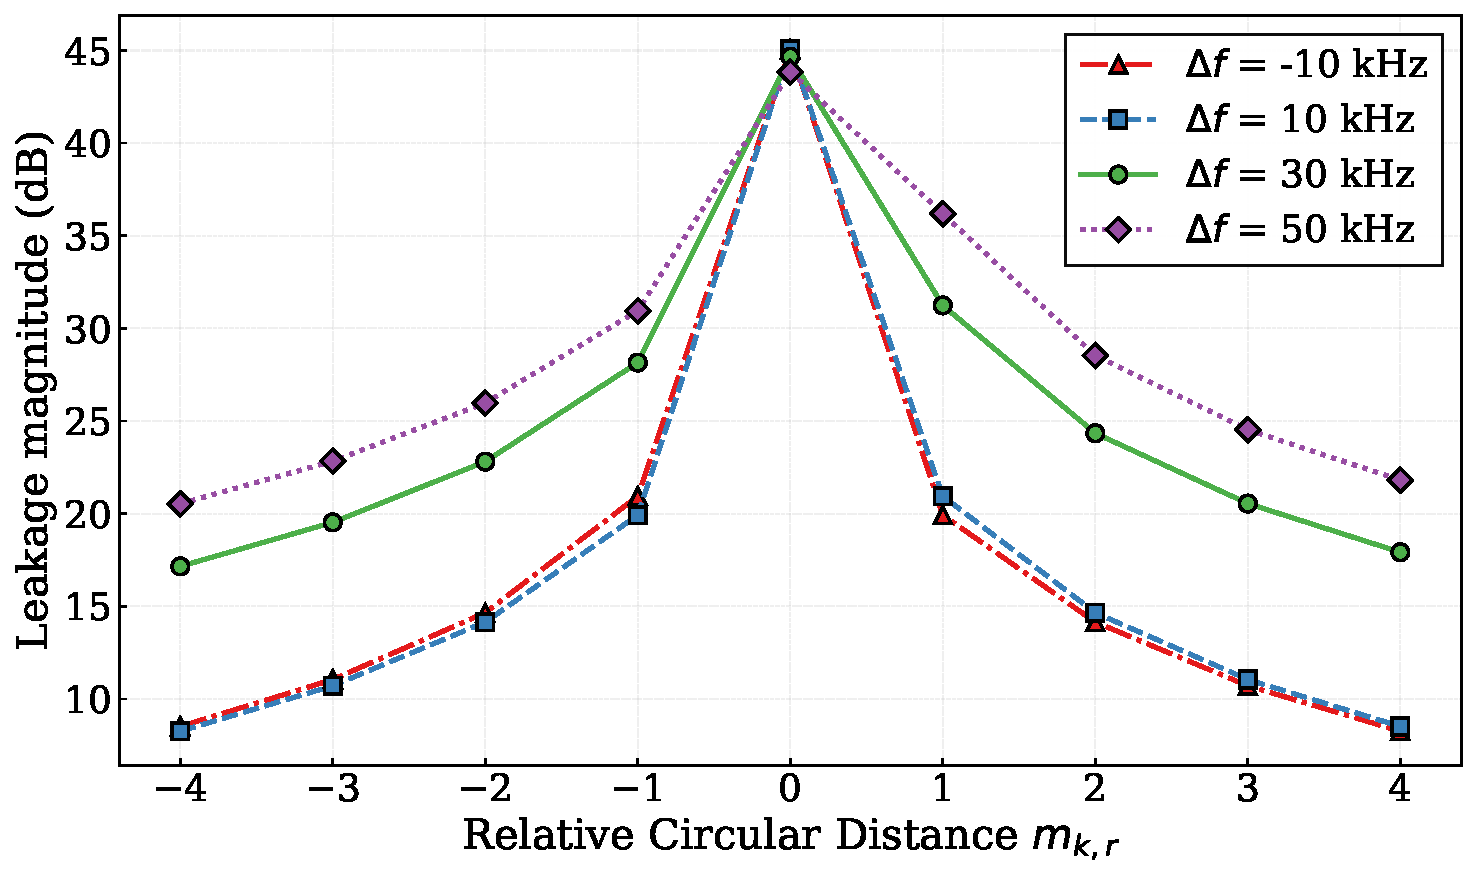
\includegraphics[width=0.8\linewidth]{fig/CFO_influence.pdf}
    \caption{Relation between magnitude of adjacent leakage and relative circular distance.}
    \label{fig:CFO_influence}
\end{figure}

\nc{Discussion, Leakage-Region Size Analysis, Page 8}
{
According to (20) and (23), the subcarrier locations of image and central leakage can be directly determined. However, adjacent leakage can spread across multiple subcarriers. Therefore, it is necessary to discuss the appropriate region size for adjacent leakage.

For a target subcarrier $k$, the leakage $L_{r\rightarrow k}
$ contributed by source subcarrier $r$ can be written as
\begin{equation}
L_{r\rightarrow k}
=
|F[m_{k,r}]|\cdot |X_{BB}[r]|,
\quad
m_{k,r}=(k-r)\bmod K,
\tag{42}
\label{eq:leakage_strength_maintext}
\end{equation}
where $m_{k,r}$ denotes the relative circular distance between the source and target subcarriers.

The CFO-induced leakage kernel is mainly controlled by this relative distance. 
Its magnitude can be written as
\begin{equation}
\left| F[m_{k,r}] \right|
=
\left|
\frac{\sin(\pi\varepsilon)}
{\sin\!\left(\frac{\pi}{K}(\varepsilon-m_{k,r})\right)}
\right|,
\quad
\varepsilon = K\Delta f T_s.
\tag{43}
\label{eq:leakage_strength_closed_form}
\end{equation}
Under the small-CFO condition and for local spectral distances, \eqref{eq:leakage_strength_closed_form} can be approximated as
\begin{equation}
|F[m_{k,r}]|
\approx
\frac{K|\varepsilon|}{|\varepsilon-m_{k,r}|}.
\tag{44}
\label{eq:F_m_small_cfo}
\end{equation}

\eqref{eq:F_m_small_cfo} shows that the adjacent leakage magnitude decreases as the relative circular distance $m_{k,r}$ increases. 
The parameter $D_a$ specifies the maximum distance from the source subcarrier included in the adjacent leakage region. As shown in Fig.~\ref{fig:CFO_influence}, the nearest neighboring subcarriers also contain the strongest leakage. Increasing $D_a$ mainly introduces weaker leakage from more distant subcarriers, together with additional computational and memory costs and possible interference from other source subcarriers. Therefore, we set $D_a=1$, corresponding to the source subcarrier and its nearest neighbor on each side.
}
}

\secc{Comment 8:}{What do you mean 40 dB AWGN? Is this the SNR or the power of the noise? Please clarify.
}

\secr{Response:}{Thank you for the comment. The ``40 dB AWGN training set'' refers to training samples with an SNR of 40 dB. At this high SNR, the noise power is much lower than the signal power. Therefore, these samples are treated as relatively clean signals for model training. We have clarified this meaning in the revised manuscript.

To clarify it, we have improved the paper as follows.

\nc{Experiment and Results, Experimental Setup, Page 9}
{The training data simulate transmission over a high-SNR channel under laboratory conditions, where AWGN is added at an SNR of 40 dB to generate samples with negligible noise.}
}

\secc{Comment 9:}{Table III, it might be easier to read by showing a delta of performance of the situation with vs without the usage of ILA-D, that way is in my opinion more immediate.
}

\secr{Response:}{Thank you for this helpful suggestion. We have revised Table~III, making the performance improvement more direct and easier to compare.

To clarify it, we have improved the paper as follows.


\setcounter{table}{2}
\begin{table*}[t]
\centering
\caption{Identification accuracy with ILA-D and the corresponding accuracy gains over the schemes without ILA-D under different SNRs.}
\label{tab:snr_results_final}
\resizebox{0.75\textwidth}{!}{
\begin{tabular}{l|l|ccccccc}
\toprule
\multicolumn{2}{c|}{Schemes} & \multicolumn{7}{c}{SNR (dB)} \\
\cmidrule(lr){1-2} \cmidrule(lr){3-9}
Classifier & Metric
& -10 & -4 & 0 & 4 & 8 & 14 & 20 \\
\midrule

Transformer [21]
& Accuracy
& 25.19\% & 53.69\% & 77.63\% & 89.56\% & 95.88\% & 98.44\% & 99.38\% \\
& $\Delta$
& +12.69\% & +39.06\% & +59.94\% & +61.31\% & +46.07\% & +7.88\% & +0.63\% \\

\midrule
ResNet18 [22]
& Accuracy
& 25.56\% & 53.19\% & 77.75\% & 89.69\% & 93.06\% & 95.56\% & 95.69\% \\
& $\Delta$
& +13.06\% & +40.69\% & +65.25\% & +77.19\% & +58.06\% & +5.43\% & +0.31\% \\

\midrule
DNN [9]
& Accuracy
& 27.44\% & 56.06\% & 81.19\% & 91.63\% & 96.44\% & 99.81\% & 100.00\% \\
& $\Delta$
& +14.94\% & +43.56\% & +68.31\% & +79.13\% & +67.06\% & +73.93\% & +0.00\% \\

\midrule
AlexNet [33]
& Accuracy
& 29.19\% & 56.06\% & 78.06\% & 89.88\% & 95.31\% & 99.13\% & 100.00\% \\
& $\Delta$
& \textbf{+16.56\%} & \textbf{+45.93\%} & +67.81\% & \textbf{+84.00\%} & +34.75\% & +1.07\% & +0.00\% \\

\midrule
LSTM-FCN [34]
& Accuracy
& 26.56\% & 57.31\% & 81.63\% & 93.50\% & 96.63\% & 98.13\% & 98.69\% \\
& $\Delta$
& +14.06\% & +44.81\% & \textbf{+69.13\%} & +71.44\% & +71.88\% & \textbf{+85.63\%} & \textbf{+70.31\%} \\

\midrule
GRU-FCN [35]
& Accuracy
& 27.38\% & 57.94\% & 80.69\% & 92.88\% & 95.00\% & 95.94\% & 97.38\% \\
& $\Delta$
& +14.88\% & +45.44\% & +68.19\% & +68.44\% & \textbf{+82.50\%} & +70.94\% & +62.82\% \\

\bottomrule
\end{tabular}
}
\parbox{\linewidth}{\vspace{2mm}\small
The Accuracy rows report the identification accuracy obtained with ILA-D.
The $\Delta$ rows report the absolute identification accuracy gain over the corresponding result without ILA-D, calculated as
$\Delta=\mathrm{Acc}_{\mathrm{w/}}-\mathrm{Acc}_{\mathrm{w/o}}$.
Values in bold indicate the largest accuracy gain among the evaluated classifiers under each SNR condition.}
\end{table*}


\nc{Experiment and Results, Tab.~\ref{tab:snr_results_final}, Page 11}
{As shown in Tab.~\ref{tab:snr_results_final}, ILA-D consistently improves all classifiers under low and moderate SNR conditions. 
At 0 dB, the accuracy gains range from $59.94 \%$ to $69.13 \%$, with LSTM-FCN achieving the largest gain. 
At higher SNRs, the gain becomes smaller for classifiers that can already achieve high accuracy without denoising, whereas ILA-D still provides substantial improvements for classifiers whose baseline performance remains limited.}
}

\secc{Comment 10:}{Perhaps I missed it, but is the system so to say adaptive, can it react to changes in the out of band responses of devices that may happen due to phenomena like aging or thermal stress? Can those change the out of band emissions so that the proposed system becomes less effective?
}

\secr{Response:}{Thank you for this comment. In this paper, adaptivity refers to the ability of ILA-D to handle varying noise levels. For noisy input signals whose SNR varies within the considered range, the ILA-aided noise prediction network estimates and suppresses the noise component to restore signals while preserving transmitter-specific impairment features. 

We agree that RFF may be affected not only by channel noise, but also by device-state and environmental factors such as aging and thermal stress. Since RFF features originate from hardware impairments, changes in the operating condition of RF components may lead to variations in the observed fingerprint distribution.
Prior studies have shown that temperature variation can cause fingerprint drift and degrade RFF classification performance when the training and testing temperatures are mismatched [1]. Recent temperature-aware RFF works also suggest that incorporating temperature information can improve generalization under temperature-varying conditions [2], [3]. These results indicate that device-state variations are important for practical RFF deployment.

In this paper, our focus is different and complementary. We mainly address the low-SNR RFF problem, where weak transmitter-specific impairment features are easily overwhelmed by noise. To this end, the proposed ILA-D exploits both in-band signals and informative out-of-band impairment leakage for diffusion-based denoising. Aging and thermal stress are beyond the main scope of the current work. We have clarified this point and added related discussion in the revised manuscript.

For practical deployment, if long-term aging or other operating-condition changes cause a significant drift from the original enrollment distribution, the system may need periodic recalibration, incremental fine-tuning, or device re-enrollment. If the relevant factors are measurable or can be approximately estimated, such as device temperature or aging stage, they may be introduced into the model as auxiliary information, condition labels, or domain variables.

Under this setting, ILA-D could be extended to a condition-aware denoising framework, where the noise prediction network is conditioned not only on the noisy in-band signal and OOB impairment leakage, but also on available device-state information. This may help the model better separate device-specific fingerprint features from state-induced variations. In addition, since out-of-band impairment leakage is generated by transmitter hardware impairments, it may provide useful complementary information for modeling state-dependent fingerprint variations. Extending ILA-D toward temperature-aware, aging-aware, or more general condition-aware RFF denoising is an interesting and practical direction for future work.


[1] Ö. Yılmaz and M. A. Yazıcı, “The Effect of Ambient Temperature On Device Classification Based On Radio Frequency Fingerprint Recognition”, SAUCIS, vol. 5, no. 2, pp. 233–245, Aug. 2022.

[2] H. Albousayri and B. Hamdaoui, “Characterizing and Mitigating the Effects of Device Temperature on RF Fingerprinting Accuracy,” arXiv:2607.25070, 2026.

[3] X. Gu, W. Wu, A. Song, M. Yang, Z. Ling, and J. Luo, “RF-TESI: Radio frequency fingerprint-based smartphone identification under temperature variation,” ACM Trans. Sensor Netw., vol. 20, no. 2, Art. no. 41, pp. 1–21, Mar. 2024.


To clarify it, we have improved the paper as follows.

\nc{Discussion, Long-Term Deployment Considerations, Page 9}
{Beyond computational efficiency, RFF may also be affected by device-state and environmental factors such as aging and thermal stress. Since RFF features originate from hardware impairments, changes in RF component conditions may alter the observed fingerprint distribution. Previous studies have shown that temperature mismatch between training and testing can degrade RFF classification performance, while incorporating temperature information can improve generalization under varying temperature conditions~[29]-[31].

If aging or other operating-condition changes cause significant deviation from the original enrollment distribution, periodic recalibration, incremental fine-tuning, or device re-enrollment may be required. When the relevant device-state factors are available, they can be introduced as auxiliary information, condition labels, or domain variables. Accordingly, ILA-D could be extended to a condition-aware denoising framework in which the noise prediction network incorporates the noisy signal, selected OOB subcarriers, and available device-state information. This extension may improve the modeling of state-dependent fingerprint variations and will be investigated in future work.}

}

% \bibliographystyle{ieeetr}
% \bibliography{bib}

\end{document}
